%
% main.tex -- Paper zum Thema Laguerre-Polynome
%
% (c) 2020 Hochschule Rapperswil
%
\chapter{Laguerre-Polynome\label{chapter:laguerre}}
\lhead{Laguerre-Polynome}
\rhead{Approximation der Gamma-Funktion}
\begin{refsection}
\chapterauthor{Patrik Müller}
\index{Patrik Müller}%
\index{Müller, Patrik}%

{\parindent0pt Die} Laguerre\--Polynome,
benannt nach Edmond Laguerre (1834 -- 1886),
\index{Edmon Laguerre}%
\index{Laguerre, Edmon}%
sind Lösungen der ebenfalls nach %Laguerre 
ihm
benannten Differentialgleichung.
Laguerre entdeckte diese Polynome, als er Appro\-xi\-ma\-tions\-methoden
für das Integral
% $\int_0^\infty \exp(-x) / x \, dx $ 
\begin{align*}
\int_0^\infty \frac{e^{-x}}{x} \, dx
\end{align*}
suchte.
Darum möchten wir uns in diesem Kapitel,
ganz im Sinne des Entdeckers,
den Laguerre-Polynomen für Approximationen von Integralen mit
exponentiell abfallenden Funktionen widmen.
Namentlich werden wir versuchen, mittels Laguerre-Polynomen und
der Gauss-Quadratur eine geeignete Approximation für die Gamma-Funktion zu
\index{Gauss-Quadratur}%
\index{Gamma-Funktion}%
finden.

Laguerre-Polynome tauchen zudem auch in der Quantenmechanik im radialen Anteil
der Lösung für die Schrödinger-Gleichung eines Wasserstoffatoms auf.
\index{Schrödinger-Gleichung}%
\index{Wasserstoffatom}%

%
% definition.tex 
%
% (c) 2022 Patrik Müller, Ostschweizer Fachhochschule
%
\section{Definition
  \label{laguerre:section:definition}}
\rhead{Definition}
Die verallgemeinerte Laguerre-Differentialgleichung ist gegeben durch
\begin{align}
x y''(x) + (\nu + 1 - x) y'(x) + n y(x)
=
0
, \quad
n \in \mathbb{N}_0
, \quad
x \in \mathbb{R}
.
\label{laguerre:dgl}
\end{align}
Spannenderweise wurde die verallgemeinerte Laguerre-Differentialgleichung
zuerst von Yacovlevich Sonine (1849 - 1915) beschrieben,
aber auf Grund ihrer Ähnlichkeit wurde sie nach Laguerre benannt.
Die klassische Laguerre-Diffentialgleichung erhält man, wenn $\nu = 0$.
Hier wird die verallgemeinerte Laguerre-Differentialgleichung verwendet,
weil die Lösung mit der selben Methode berechnet werden kann,
aber man zusätzlich die Lösung für den allgmeinen Fall erhält.
Zur Lösung von \eqref{laguerre:dgl} verwenden wir einen
Potenzreihenansatz.
Da wir bereits wissen, dass die Lösung orthogonale Polynome sind,
erscheint dieser Ansatz sinnvoll.
Setzt man nun den Ansatz
\begin{align*}
y(x)
 & =
\sum_{k=0}^\infty a_k x^k
\\
y'(x)
 & =
\sum_{k=1}^\infty k a_k x^{k-1}
=
\sum_{k=0}^\infty (k+1) a_{k+1} x^k
\\
y''(x)
 & =
\sum_{k=2}^\infty k (k-1) a_k x^{k-2}
=
\sum_{k=1}^\infty (k+1) k a_{k+1} x^{k-1}
\end{align*}
in die Differentialgleichung ein, erhält man:
\begin{align*}
\sum_{k=1}^\infty (k+1) k a_{k+1} x^k
+
(\nu + 1)\sum_{k=0}^\infty (k+1) a_{k+1} x^k
-
\sum_{k=0}^\infty k a_k x^k
+
n \sum_{k=0}^\infty a_k x^k
 & =
0    \\
\sum_{k=1}^\infty
\left[ (k+1) k a_{k+1} + (\nu + 1)(k+1) a_{k+1} - k a_k + n a_k \right] x^k
 & =
0.
\end{align*}
Daraus lässt sich die Rekursionsbeziehung
\begin{align*}
a_{k+1}
 & =
\frac{k-n}{(k+1) (k + \nu + 1)} a_k
\end{align*}
ableiten.
Für ein konstantes $n$ erhalten wir als Potenzreihenlösung ein Polynom vom Grad
$n$,
denn für $k=n$ wird $a_{n+1} = 0$ und damit auch $a_{n+2}=a_{n+3}=\ldots=0$.
Aus der Rekursionsbeziehung ist zudem ersichtlich,
dass $a_0 \neq 0$ beliebig gewählt werden kann.
Wählen wir nun $a_0 = 1$, dann folgt für die Koeffizienten $a_1, a_2, a_3$
\begin{align*}
a_1
=
-\frac{n}{1 \cdot (\nu + 1)}
, &  &
a_2
=
\frac{(n-1)n}{1 \cdot 2 \cdot (\nu + 1)(\nu + 2)}
, &  &
a_3
=
-\frac{(n-2)(n-1)n}{1 \cdot 2 \cdot 3 \cdot (\nu + 1)(\nu + 2)(\nu + 3)}
\end{align*}
und allgemein
\begin{align*}
k
  & \leq
n:
  &
a_k
  & =
(-1)^k \frac{n!}{(n-k)!} \frac{1}{k!(\nu + 1)_k}
=
\frac{(-1)^k}{(\nu + 1)_k} \binom{n}{k}
\\
k & >n:
  &
a_k
  & =
0.
\end{align*}
Somit erhalten wir für $\nu = 0$ die Laguerre-Polynome
\begin{align}
L_n(x)
=
\sum_{k=0}^{n} \frac{(-1)^k}{k!} \binom{n}{k} x^k
\label{laguerre:polynom}
\end{align}
und mit $\nu \in \mathbb{R}$ die verallgemeinerten Laguerre-Polynome
\begin{align}
L_n^\nu(x)
=
\sum_{k=0}^{n} \frac{(-1)^k}{(\nu + 1)_k} \binom{n}{k} x^k.
\label{laguerre:allg_polynom}
\end{align}
Die Laguerre-Polynome von Grad $0$ bis $7$ sind in
Abbildung~\ref{laguerre:fig:polyeval} dargestellt.
\begin{figure}
\centering
\scalebox{0.8}{%% Creator: Matplotlib, PGF backend
%%
%% To include the figure in your LaTeX document, write
%%   \input{<filename>.pgf}
%%
%% Make sure the required packages are loaded in your preamble
%%   \usepackage{pgf}
%%
%% Also ensure that all the required font packages are loaded; for instance,
%% the lmodern package is sometimes necessary when using math font.
%%   \usepackage{lmodern}
%%
%% Figures using additional raster images can only be included by \input if
%% they are in the same directory as the main LaTeX file. For loading figures
%% from other directories you can use the `import` package
%%   \usepackage{import}
%%
%% and then include the figures with
%%   \import{<path to file>}{<filename>.pgf}
%%
%% Matplotlib used the following preamble
%%   \usepackage{fontspec}
%%   \setmainfont{DejaVuSerif.ttf}[Path=\detokenize{/home/mup/.local/lib/python3.8/site-packages/matplotlib/mpl-data/fonts/ttf/}]
%%   \setsansfont{DejaVuSans.ttf}[Path=\detokenize{/home/mup/.local/lib/python3.8/site-packages/matplotlib/mpl-data/fonts/ttf/}]
%%   \setmonofont{DejaVuSansMono.ttf}[Path=\detokenize{/home/mup/.local/lib/python3.8/site-packages/matplotlib/mpl-data/fonts/ttf/}]
%%
\begingroup%
\makeatletter%
\begin{pgfpicture}%
\pgfpathrectangle{\pgfpointorigin}{\pgfqpoint{6.000000in}{4.000000in}}%
\pgfusepath{use as bounding box, clip}%
\begin{pgfscope}%
\pgfsetbuttcap%
\pgfsetmiterjoin%
\definecolor{currentfill}{rgb}{1.000000,1.000000,1.000000}%
\pgfsetfillcolor{currentfill}%
\pgfsetlinewidth{0.000000pt}%
\definecolor{currentstroke}{rgb}{1.000000,1.000000,1.000000}%
\pgfsetstrokecolor{currentstroke}%
\pgfsetdash{}{0pt}%
\pgfpathmoveto{\pgfqpoint{0.000000in}{0.000000in}}%
\pgfpathlineto{\pgfqpoint{6.000000in}{0.000000in}}%
\pgfpathlineto{\pgfqpoint{6.000000in}{4.000000in}}%
\pgfpathlineto{\pgfqpoint{0.000000in}{4.000000in}}%
\pgfpathlineto{\pgfqpoint{0.000000in}{0.000000in}}%
\pgfpathclose%
\pgfusepath{fill}%
\end{pgfscope}%
\begin{pgfscope}%
\pgfsetbuttcap%
\pgfsetmiterjoin%
\definecolor{currentfill}{rgb}{1.000000,1.000000,1.000000}%
\pgfsetfillcolor{currentfill}%
\pgfsetlinewidth{0.000000pt}%
\definecolor{currentstroke}{rgb}{0.000000,0.000000,0.000000}%
\pgfsetstrokecolor{currentstroke}%
\pgfsetstrokeopacity{0.000000}%
\pgfsetdash{}{0pt}%
\pgfpathmoveto{\pgfqpoint{0.041670in}{0.041670in}}%
\pgfpathlineto{\pgfqpoint{5.953330in}{0.041670in}}%
\pgfpathlineto{\pgfqpoint{5.953330in}{3.958330in}}%
\pgfpathlineto{\pgfqpoint{0.041670in}{3.958330in}}%
\pgfpathlineto{\pgfqpoint{0.041670in}{0.041670in}}%
\pgfpathclose%
\pgfusepath{fill}%
\end{pgfscope}%
\begin{pgfscope}%
\pgfsetbuttcap%
\pgfsetmiterjoin%
\definecolor{currentfill}{rgb}{0.000000,0.000000,0.000000}%
\pgfsetfillcolor{currentfill}%
\pgfsetlinewidth{0.501875pt}%
\definecolor{currentstroke}{rgb}{0.000000,0.000000,0.000000}%
\pgfsetstrokecolor{currentstroke}%
\pgfsetdash{}{0pt}%
\pgfpathmoveto{\pgfqpoint{5.952738in}{2.000000in}}%
\pgfpathlineto{\pgfqpoint{5.755703in}{1.967361in}}%
\pgfpathlineto{\pgfqpoint{5.755703in}{1.999925in}}%
\pgfpathlineto{\pgfqpoint{5.755703in}{1.999925in}}%
\pgfpathlineto{\pgfqpoint{5.755703in}{2.000075in}}%
\pgfpathlineto{\pgfqpoint{5.755703in}{2.000075in}}%
\pgfpathlineto{\pgfqpoint{5.755703in}{2.032639in}}%
\pgfpathlineto{\pgfqpoint{5.952738in}{2.000000in}}%
\pgfpathclose%
\pgfusepath{stroke,fill}%
\end{pgfscope}%
\begin{pgfscope}%
\pgfsetbuttcap%
\pgfsetmiterjoin%
\definecolor{currentfill}{rgb}{0.000000,0.000000,0.000000}%
\pgfsetfillcolor{currentfill}%
\pgfsetlinewidth{0.501875pt}%
\definecolor{currentstroke}{rgb}{0.000000,0.000000,0.000000}%
\pgfsetstrokecolor{currentstroke}%
\pgfsetdash{}{0pt}%
\pgfpathmoveto{\pgfqpoint{0.579040in}{3.958330in}}%
\pgfpathlineto{\pgfqpoint{0.611667in}{3.761225in}}%
\pgfpathlineto{\pgfqpoint{0.579296in}{3.761225in}}%
\pgfpathlineto{\pgfqpoint{0.579296in}{3.761225in}}%
\pgfpathlineto{\pgfqpoint{0.578784in}{3.761225in}}%
\pgfpathlineto{\pgfqpoint{0.578784in}{3.761225in}}%
\pgfpathlineto{\pgfqpoint{0.546412in}{3.761225in}}%
\pgfpathlineto{\pgfqpoint{0.579040in}{3.958330in}}%
\pgfpathclose%
\pgfusepath{stroke,fill}%
\end{pgfscope}%
\begin{pgfscope}%
\pgfsetbuttcap%
\pgfsetroundjoin%
\definecolor{currentfill}{rgb}{0.000000,0.000000,0.000000}%
\pgfsetfillcolor{currentfill}%
\pgfsetlinewidth{0.803000pt}%
\definecolor{currentstroke}{rgb}{0.000000,0.000000,0.000000}%
\pgfsetstrokecolor{currentstroke}%
\pgfsetdash{}{0pt}%
\pgfsys@defobject{currentmarker}{\pgfqpoint{0.000000in}{-0.048611in}}{\pgfqpoint{0.000000in}{0.000000in}}{%
\pgfpathmoveto{\pgfqpoint{0.000000in}{0.000000in}}%
\pgfpathlineto{\pgfqpoint{0.000000in}{-0.048611in}}%
\pgfusepath{stroke,fill}%
}%
\begin{pgfscope}%
\pgfsys@transformshift{3.137944in}{2.000000in}%
\pgfsys@useobject{currentmarker}{}%
\end{pgfscope}%
\end{pgfscope}%
\begin{pgfscope}%
\definecolor{textcolor}{rgb}{0.000000,0.000000,0.000000}%
\pgfsetstrokecolor{textcolor}%
\pgfsetfillcolor{textcolor}%
\pgftext[x=3.137944in,y=1.902778in,,top]{\color{textcolor}\sffamily\fontsize{10.000000}{12.000000}\selectfont 5}%
\end{pgfscope}%
\begin{pgfscope}%
\pgfsetbuttcap%
\pgfsetroundjoin%
\definecolor{currentfill}{rgb}{0.000000,0.000000,0.000000}%
\pgfsetfillcolor{currentfill}%
\pgfsetlinewidth{0.803000pt}%
\definecolor{currentstroke}{rgb}{0.000000,0.000000,0.000000}%
\pgfsetstrokecolor{currentstroke}%
\pgfsetdash{}{0pt}%
\pgfsys@defobject{currentmarker}{\pgfqpoint{0.000000in}{-0.048611in}}{\pgfqpoint{0.000000in}{0.000000in}}{%
\pgfpathmoveto{\pgfqpoint{0.000000in}{0.000000in}}%
\pgfpathlineto{\pgfqpoint{0.000000in}{-0.048611in}}%
\pgfusepath{stroke,fill}%
}%
\begin{pgfscope}%
\pgfsys@transformshift{5.696848in}{2.000000in}%
\pgfsys@useobject{currentmarker}{}%
\end{pgfscope}%
\end{pgfscope}%
\begin{pgfscope}%
\definecolor{textcolor}{rgb}{0.000000,0.000000,0.000000}%
\pgfsetstrokecolor{textcolor}%
\pgfsetfillcolor{textcolor}%
\pgftext[x=5.696848in,y=1.902778in,,top]{\color{textcolor}\sffamily\fontsize{10.000000}{12.000000}\selectfont 10}%
\end{pgfscope}%
\begin{pgfscope}%
\pgfsetbuttcap%
\pgfsetroundjoin%
\definecolor{currentfill}{rgb}{0.000000,0.000000,0.000000}%
\pgfsetfillcolor{currentfill}%
\pgfsetlinewidth{0.602250pt}%
\definecolor{currentstroke}{rgb}{0.000000,0.000000,0.000000}%
\pgfsetstrokecolor{currentstroke}%
\pgfsetdash{}{0pt}%
\pgfsys@defobject{currentmarker}{\pgfqpoint{0.000000in}{-0.027778in}}{\pgfqpoint{0.000000in}{0.000000in}}{%
\pgfpathmoveto{\pgfqpoint{0.000000in}{0.000000in}}%
\pgfpathlineto{\pgfqpoint{0.000000in}{-0.027778in}}%
\pgfusepath{stroke,fill}%
}%
\begin{pgfscope}%
\pgfsys@transformshift{0.067259in}{2.000000in}%
\pgfsys@useobject{currentmarker}{}%
\end{pgfscope}%
\end{pgfscope}%
\begin{pgfscope}%
\pgfsetbuttcap%
\pgfsetroundjoin%
\definecolor{currentfill}{rgb}{0.000000,0.000000,0.000000}%
\pgfsetfillcolor{currentfill}%
\pgfsetlinewidth{0.602250pt}%
\definecolor{currentstroke}{rgb}{0.000000,0.000000,0.000000}%
\pgfsetstrokecolor{currentstroke}%
\pgfsetdash{}{0pt}%
\pgfsys@defobject{currentmarker}{\pgfqpoint{0.000000in}{-0.027778in}}{\pgfqpoint{0.000000in}{0.000000in}}{%
\pgfpathmoveto{\pgfqpoint{0.000000in}{0.000000in}}%
\pgfpathlineto{\pgfqpoint{0.000000in}{-0.027778in}}%
\pgfusepath{stroke,fill}%
}%
\begin{pgfscope}%
\pgfsys@transformshift{1.090821in}{2.000000in}%
\pgfsys@useobject{currentmarker}{}%
\end{pgfscope}%
\end{pgfscope}%
\begin{pgfscope}%
\pgfsetbuttcap%
\pgfsetroundjoin%
\definecolor{currentfill}{rgb}{0.000000,0.000000,0.000000}%
\pgfsetfillcolor{currentfill}%
\pgfsetlinewidth{0.602250pt}%
\definecolor{currentstroke}{rgb}{0.000000,0.000000,0.000000}%
\pgfsetstrokecolor{currentstroke}%
\pgfsetdash{}{0pt}%
\pgfsys@defobject{currentmarker}{\pgfqpoint{0.000000in}{-0.027778in}}{\pgfqpoint{0.000000in}{0.000000in}}{%
\pgfpathmoveto{\pgfqpoint{0.000000in}{0.000000in}}%
\pgfpathlineto{\pgfqpoint{0.000000in}{-0.027778in}}%
\pgfusepath{stroke,fill}%
}%
\begin{pgfscope}%
\pgfsys@transformshift{1.602601in}{2.000000in}%
\pgfsys@useobject{currentmarker}{}%
\end{pgfscope}%
\end{pgfscope}%
\begin{pgfscope}%
\pgfsetbuttcap%
\pgfsetroundjoin%
\definecolor{currentfill}{rgb}{0.000000,0.000000,0.000000}%
\pgfsetfillcolor{currentfill}%
\pgfsetlinewidth{0.602250pt}%
\definecolor{currentstroke}{rgb}{0.000000,0.000000,0.000000}%
\pgfsetstrokecolor{currentstroke}%
\pgfsetdash{}{0pt}%
\pgfsys@defobject{currentmarker}{\pgfqpoint{0.000000in}{-0.027778in}}{\pgfqpoint{0.000000in}{0.000000in}}{%
\pgfpathmoveto{\pgfqpoint{0.000000in}{0.000000in}}%
\pgfpathlineto{\pgfqpoint{0.000000in}{-0.027778in}}%
\pgfusepath{stroke,fill}%
}%
\begin{pgfscope}%
\pgfsys@transformshift{2.114382in}{2.000000in}%
\pgfsys@useobject{currentmarker}{}%
\end{pgfscope}%
\end{pgfscope}%
\begin{pgfscope}%
\pgfsetbuttcap%
\pgfsetroundjoin%
\definecolor{currentfill}{rgb}{0.000000,0.000000,0.000000}%
\pgfsetfillcolor{currentfill}%
\pgfsetlinewidth{0.602250pt}%
\definecolor{currentstroke}{rgb}{0.000000,0.000000,0.000000}%
\pgfsetstrokecolor{currentstroke}%
\pgfsetdash{}{0pt}%
\pgfsys@defobject{currentmarker}{\pgfqpoint{0.000000in}{-0.027778in}}{\pgfqpoint{0.000000in}{0.000000in}}{%
\pgfpathmoveto{\pgfqpoint{0.000000in}{0.000000in}}%
\pgfpathlineto{\pgfqpoint{0.000000in}{-0.027778in}}%
\pgfusepath{stroke,fill}%
}%
\begin{pgfscope}%
\pgfsys@transformshift{2.626163in}{2.000000in}%
\pgfsys@useobject{currentmarker}{}%
\end{pgfscope}%
\end{pgfscope}%
\begin{pgfscope}%
\pgfsetbuttcap%
\pgfsetroundjoin%
\definecolor{currentfill}{rgb}{0.000000,0.000000,0.000000}%
\pgfsetfillcolor{currentfill}%
\pgfsetlinewidth{0.602250pt}%
\definecolor{currentstroke}{rgb}{0.000000,0.000000,0.000000}%
\pgfsetstrokecolor{currentstroke}%
\pgfsetdash{}{0pt}%
\pgfsys@defobject{currentmarker}{\pgfqpoint{0.000000in}{-0.027778in}}{\pgfqpoint{0.000000in}{0.000000in}}{%
\pgfpathmoveto{\pgfqpoint{0.000000in}{0.000000in}}%
\pgfpathlineto{\pgfqpoint{0.000000in}{-0.027778in}}%
\pgfusepath{stroke,fill}%
}%
\begin{pgfscope}%
\pgfsys@transformshift{3.649725in}{2.000000in}%
\pgfsys@useobject{currentmarker}{}%
\end{pgfscope}%
\end{pgfscope}%
\begin{pgfscope}%
\pgfsetbuttcap%
\pgfsetroundjoin%
\definecolor{currentfill}{rgb}{0.000000,0.000000,0.000000}%
\pgfsetfillcolor{currentfill}%
\pgfsetlinewidth{0.602250pt}%
\definecolor{currentstroke}{rgb}{0.000000,0.000000,0.000000}%
\pgfsetstrokecolor{currentstroke}%
\pgfsetdash{}{0pt}%
\pgfsys@defobject{currentmarker}{\pgfqpoint{0.000000in}{-0.027778in}}{\pgfqpoint{0.000000in}{0.000000in}}{%
\pgfpathmoveto{\pgfqpoint{0.000000in}{0.000000in}}%
\pgfpathlineto{\pgfqpoint{0.000000in}{-0.027778in}}%
\pgfusepath{stroke,fill}%
}%
\begin{pgfscope}%
\pgfsys@transformshift{4.161505in}{2.000000in}%
\pgfsys@useobject{currentmarker}{}%
\end{pgfscope}%
\end{pgfscope}%
\begin{pgfscope}%
\pgfsetbuttcap%
\pgfsetroundjoin%
\definecolor{currentfill}{rgb}{0.000000,0.000000,0.000000}%
\pgfsetfillcolor{currentfill}%
\pgfsetlinewidth{0.602250pt}%
\definecolor{currentstroke}{rgb}{0.000000,0.000000,0.000000}%
\pgfsetstrokecolor{currentstroke}%
\pgfsetdash{}{0pt}%
\pgfsys@defobject{currentmarker}{\pgfqpoint{0.000000in}{-0.027778in}}{\pgfqpoint{0.000000in}{0.000000in}}{%
\pgfpathmoveto{\pgfqpoint{0.000000in}{0.000000in}}%
\pgfpathlineto{\pgfqpoint{0.000000in}{-0.027778in}}%
\pgfusepath{stroke,fill}%
}%
\begin{pgfscope}%
\pgfsys@transformshift{4.673286in}{2.000000in}%
\pgfsys@useobject{currentmarker}{}%
\end{pgfscope}%
\end{pgfscope}%
\begin{pgfscope}%
\pgfsetbuttcap%
\pgfsetroundjoin%
\definecolor{currentfill}{rgb}{0.000000,0.000000,0.000000}%
\pgfsetfillcolor{currentfill}%
\pgfsetlinewidth{0.602250pt}%
\definecolor{currentstroke}{rgb}{0.000000,0.000000,0.000000}%
\pgfsetstrokecolor{currentstroke}%
\pgfsetdash{}{0pt}%
\pgfsys@defobject{currentmarker}{\pgfqpoint{0.000000in}{-0.027778in}}{\pgfqpoint{0.000000in}{0.000000in}}{%
\pgfpathmoveto{\pgfqpoint{0.000000in}{0.000000in}}%
\pgfpathlineto{\pgfqpoint{0.000000in}{-0.027778in}}%
\pgfusepath{stroke,fill}%
}%
\begin{pgfscope}%
\pgfsys@transformshift{5.185067in}{2.000000in}%
\pgfsys@useobject{currentmarker}{}%
\end{pgfscope}%
\end{pgfscope}%
\begin{pgfscope}%
\definecolor{textcolor}{rgb}{0.000000,0.000000,0.000000}%
\pgfsetstrokecolor{textcolor}%
\pgfsetfillcolor{textcolor}%
\pgftext[x=5.953330in,y=1.907254in,,top]{\color{textcolor}\sffamily\fontsize{12.000000}{14.400000}\selectfont \(\displaystyle x\)}%
\end{pgfscope}%
\begin{pgfscope}%
\pgfsetbuttcap%
\pgfsetroundjoin%
\definecolor{currentfill}{rgb}{0.000000,0.000000,0.000000}%
\pgfsetfillcolor{currentfill}%
\pgfsetlinewidth{0.803000pt}%
\definecolor{currentstroke}{rgb}{0.000000,0.000000,0.000000}%
\pgfsetstrokecolor{currentstroke}%
\pgfsetdash{}{0pt}%
\pgfsys@defobject{currentmarker}{\pgfqpoint{-0.048611in}{0.000000in}}{\pgfqpoint{-0.000000in}{0.000000in}}{%
\pgfpathmoveto{\pgfqpoint{-0.000000in}{0.000000in}}%
\pgfpathlineto{\pgfqpoint{-0.048611in}{0.000000in}}%
\pgfusepath{stroke,fill}%
}%
\begin{pgfscope}%
\pgfsys@transformshift{0.579040in}{0.493592in}%
\pgfsys@useobject{currentmarker}{}%
\end{pgfscope}%
\end{pgfscope}%
\begin{pgfscope}%
\definecolor{textcolor}{rgb}{0.000000,0.000000,0.000000}%
\pgfsetstrokecolor{textcolor}%
\pgfsetfillcolor{textcolor}%
\pgftext[x=0.197062in, y=0.440831in, left, base]{\color{textcolor}\sffamily\fontsize{10.000000}{12.000000}\selectfont \ensuremath{-}10}%
\end{pgfscope}%
\begin{pgfscope}%
\pgfsetbuttcap%
\pgfsetroundjoin%
\definecolor{currentfill}{rgb}{0.000000,0.000000,0.000000}%
\pgfsetfillcolor{currentfill}%
\pgfsetlinewidth{0.803000pt}%
\definecolor{currentstroke}{rgb}{0.000000,0.000000,0.000000}%
\pgfsetstrokecolor{currentstroke}%
\pgfsetdash{}{0pt}%
\pgfsys@defobject{currentmarker}{\pgfqpoint{-0.048611in}{0.000000in}}{\pgfqpoint{-0.000000in}{0.000000in}}{%
\pgfpathmoveto{\pgfqpoint{-0.000000in}{0.000000in}}%
\pgfpathlineto{\pgfqpoint{-0.048611in}{0.000000in}}%
\pgfusepath{stroke,fill}%
}%
\begin{pgfscope}%
\pgfsys@transformshift{0.579040in}{1.246796in}%
\pgfsys@useobject{currentmarker}{}%
\end{pgfscope}%
\end{pgfscope}%
\begin{pgfscope}%
\definecolor{textcolor}{rgb}{0.000000,0.000000,0.000000}%
\pgfsetstrokecolor{textcolor}%
\pgfsetfillcolor{textcolor}%
\pgftext[x=0.285427in, y=1.194035in, left, base]{\color{textcolor}\sffamily\fontsize{10.000000}{12.000000}\selectfont \ensuremath{-}5}%
\end{pgfscope}%
\begin{pgfscope}%
\pgfsetbuttcap%
\pgfsetroundjoin%
\definecolor{currentfill}{rgb}{0.000000,0.000000,0.000000}%
\pgfsetfillcolor{currentfill}%
\pgfsetlinewidth{0.803000pt}%
\definecolor{currentstroke}{rgb}{0.000000,0.000000,0.000000}%
\pgfsetstrokecolor{currentstroke}%
\pgfsetdash{}{0pt}%
\pgfsys@defobject{currentmarker}{\pgfqpoint{-0.048611in}{0.000000in}}{\pgfqpoint{-0.000000in}{0.000000in}}{%
\pgfpathmoveto{\pgfqpoint{-0.000000in}{0.000000in}}%
\pgfpathlineto{\pgfqpoint{-0.048611in}{0.000000in}}%
\pgfusepath{stroke,fill}%
}%
\begin{pgfscope}%
\pgfsys@transformshift{0.579040in}{2.000000in}%
\pgfsys@useobject{currentmarker}{}%
\end{pgfscope}%
\end{pgfscope}%
\begin{pgfscope}%
\definecolor{textcolor}{rgb}{0.000000,0.000000,0.000000}%
\pgfsetstrokecolor{textcolor}%
\pgfsetfillcolor{textcolor}%
\pgftext[x=0.393452in, y=1.947238in, left, base]{\color{textcolor}\sffamily\fontsize{10.000000}{12.000000}\selectfont 0}%
\end{pgfscope}%
\begin{pgfscope}%
\pgfsetbuttcap%
\pgfsetroundjoin%
\definecolor{currentfill}{rgb}{0.000000,0.000000,0.000000}%
\pgfsetfillcolor{currentfill}%
\pgfsetlinewidth{0.803000pt}%
\definecolor{currentstroke}{rgb}{0.000000,0.000000,0.000000}%
\pgfsetstrokecolor{currentstroke}%
\pgfsetdash{}{0pt}%
\pgfsys@defobject{currentmarker}{\pgfqpoint{-0.048611in}{0.000000in}}{\pgfqpoint{-0.000000in}{0.000000in}}{%
\pgfpathmoveto{\pgfqpoint{-0.000000in}{0.000000in}}%
\pgfpathlineto{\pgfqpoint{-0.048611in}{0.000000in}}%
\pgfusepath{stroke,fill}%
}%
\begin{pgfscope}%
\pgfsys@transformshift{0.579040in}{2.753204in}%
\pgfsys@useobject{currentmarker}{}%
\end{pgfscope}%
\end{pgfscope}%
\begin{pgfscope}%
\definecolor{textcolor}{rgb}{0.000000,0.000000,0.000000}%
\pgfsetstrokecolor{textcolor}%
\pgfsetfillcolor{textcolor}%
\pgftext[x=0.393452in, y=2.700442in, left, base]{\color{textcolor}\sffamily\fontsize{10.000000}{12.000000}\selectfont 5}%
\end{pgfscope}%
\begin{pgfscope}%
\pgfsetbuttcap%
\pgfsetroundjoin%
\definecolor{currentfill}{rgb}{0.000000,0.000000,0.000000}%
\pgfsetfillcolor{currentfill}%
\pgfsetlinewidth{0.803000pt}%
\definecolor{currentstroke}{rgb}{0.000000,0.000000,0.000000}%
\pgfsetstrokecolor{currentstroke}%
\pgfsetdash{}{0pt}%
\pgfsys@defobject{currentmarker}{\pgfqpoint{-0.048611in}{0.000000in}}{\pgfqpoint{-0.000000in}{0.000000in}}{%
\pgfpathmoveto{\pgfqpoint{-0.000000in}{0.000000in}}%
\pgfpathlineto{\pgfqpoint{-0.048611in}{0.000000in}}%
\pgfusepath{stroke,fill}%
}%
\begin{pgfscope}%
\pgfsys@transformshift{0.579040in}{3.506408in}%
\pgfsys@useobject{currentmarker}{}%
\end{pgfscope}%
\end{pgfscope}%
\begin{pgfscope}%
\definecolor{textcolor}{rgb}{0.000000,0.000000,0.000000}%
\pgfsetstrokecolor{textcolor}%
\pgfsetfillcolor{textcolor}%
\pgftext[x=0.305087in, y=3.453646in, left, base]{\color{textcolor}\sffamily\fontsize{10.000000}{12.000000}\selectfont 10}%
\end{pgfscope}%
\begin{pgfscope}%
\pgfsetbuttcap%
\pgfsetroundjoin%
\definecolor{currentfill}{rgb}{0.000000,0.000000,0.000000}%
\pgfsetfillcolor{currentfill}%
\pgfsetlinewidth{0.602250pt}%
\definecolor{currentstroke}{rgb}{0.000000,0.000000,0.000000}%
\pgfsetstrokecolor{currentstroke}%
\pgfsetdash{}{0pt}%
\pgfsys@defobject{currentmarker}{\pgfqpoint{-0.027778in}{0.000000in}}{\pgfqpoint{-0.000000in}{0.000000in}}{%
\pgfpathmoveto{\pgfqpoint{-0.000000in}{0.000000in}}%
\pgfpathlineto{\pgfqpoint{-0.027778in}{0.000000in}}%
\pgfusepath{stroke,fill}%
}%
\begin{pgfscope}%
\pgfsys@transformshift{0.579040in}{0.041670in}%
\pgfsys@useobject{currentmarker}{}%
\end{pgfscope}%
\end{pgfscope}%
\begin{pgfscope}%
\pgfsetbuttcap%
\pgfsetroundjoin%
\definecolor{currentfill}{rgb}{0.000000,0.000000,0.000000}%
\pgfsetfillcolor{currentfill}%
\pgfsetlinewidth{0.602250pt}%
\definecolor{currentstroke}{rgb}{0.000000,0.000000,0.000000}%
\pgfsetstrokecolor{currentstroke}%
\pgfsetdash{}{0pt}%
\pgfsys@defobject{currentmarker}{\pgfqpoint{-0.027778in}{0.000000in}}{\pgfqpoint{-0.000000in}{0.000000in}}{%
\pgfpathmoveto{\pgfqpoint{-0.000000in}{0.000000in}}%
\pgfpathlineto{\pgfqpoint{-0.027778in}{0.000000in}}%
\pgfusepath{stroke,fill}%
}%
\begin{pgfscope}%
\pgfsys@transformshift{0.579040in}{0.192311in}%
\pgfsys@useobject{currentmarker}{}%
\end{pgfscope}%
\end{pgfscope}%
\begin{pgfscope}%
\pgfsetbuttcap%
\pgfsetroundjoin%
\definecolor{currentfill}{rgb}{0.000000,0.000000,0.000000}%
\pgfsetfillcolor{currentfill}%
\pgfsetlinewidth{0.602250pt}%
\definecolor{currentstroke}{rgb}{0.000000,0.000000,0.000000}%
\pgfsetstrokecolor{currentstroke}%
\pgfsetdash{}{0pt}%
\pgfsys@defobject{currentmarker}{\pgfqpoint{-0.027778in}{0.000000in}}{\pgfqpoint{-0.000000in}{0.000000in}}{%
\pgfpathmoveto{\pgfqpoint{-0.000000in}{0.000000in}}%
\pgfpathlineto{\pgfqpoint{-0.027778in}{0.000000in}}%
\pgfusepath{stroke,fill}%
}%
\begin{pgfscope}%
\pgfsys@transformshift{0.579040in}{0.342952in}%
\pgfsys@useobject{currentmarker}{}%
\end{pgfscope}%
\end{pgfscope}%
\begin{pgfscope}%
\pgfsetbuttcap%
\pgfsetroundjoin%
\definecolor{currentfill}{rgb}{0.000000,0.000000,0.000000}%
\pgfsetfillcolor{currentfill}%
\pgfsetlinewidth{0.602250pt}%
\definecolor{currentstroke}{rgb}{0.000000,0.000000,0.000000}%
\pgfsetstrokecolor{currentstroke}%
\pgfsetdash{}{0pt}%
\pgfsys@defobject{currentmarker}{\pgfqpoint{-0.027778in}{0.000000in}}{\pgfqpoint{-0.000000in}{0.000000in}}{%
\pgfpathmoveto{\pgfqpoint{-0.000000in}{0.000000in}}%
\pgfpathlineto{\pgfqpoint{-0.027778in}{0.000000in}}%
\pgfusepath{stroke,fill}%
}%
\begin{pgfscope}%
\pgfsys@transformshift{0.579040in}{0.644233in}%
\pgfsys@useobject{currentmarker}{}%
\end{pgfscope}%
\end{pgfscope}%
\begin{pgfscope}%
\pgfsetbuttcap%
\pgfsetroundjoin%
\definecolor{currentfill}{rgb}{0.000000,0.000000,0.000000}%
\pgfsetfillcolor{currentfill}%
\pgfsetlinewidth{0.602250pt}%
\definecolor{currentstroke}{rgb}{0.000000,0.000000,0.000000}%
\pgfsetstrokecolor{currentstroke}%
\pgfsetdash{}{0pt}%
\pgfsys@defobject{currentmarker}{\pgfqpoint{-0.027778in}{0.000000in}}{\pgfqpoint{-0.000000in}{0.000000in}}{%
\pgfpathmoveto{\pgfqpoint{-0.000000in}{0.000000in}}%
\pgfpathlineto{\pgfqpoint{-0.027778in}{0.000000in}}%
\pgfusepath{stroke,fill}%
}%
\begin{pgfscope}%
\pgfsys@transformshift{0.579040in}{0.794874in}%
\pgfsys@useobject{currentmarker}{}%
\end{pgfscope}%
\end{pgfscope}%
\begin{pgfscope}%
\pgfsetbuttcap%
\pgfsetroundjoin%
\definecolor{currentfill}{rgb}{0.000000,0.000000,0.000000}%
\pgfsetfillcolor{currentfill}%
\pgfsetlinewidth{0.602250pt}%
\definecolor{currentstroke}{rgb}{0.000000,0.000000,0.000000}%
\pgfsetstrokecolor{currentstroke}%
\pgfsetdash{}{0pt}%
\pgfsys@defobject{currentmarker}{\pgfqpoint{-0.027778in}{0.000000in}}{\pgfqpoint{-0.000000in}{0.000000in}}{%
\pgfpathmoveto{\pgfqpoint{-0.000000in}{0.000000in}}%
\pgfpathlineto{\pgfqpoint{-0.027778in}{0.000000in}}%
\pgfusepath{stroke,fill}%
}%
\begin{pgfscope}%
\pgfsys@transformshift{0.579040in}{0.945515in}%
\pgfsys@useobject{currentmarker}{}%
\end{pgfscope}%
\end{pgfscope}%
\begin{pgfscope}%
\pgfsetbuttcap%
\pgfsetroundjoin%
\definecolor{currentfill}{rgb}{0.000000,0.000000,0.000000}%
\pgfsetfillcolor{currentfill}%
\pgfsetlinewidth{0.602250pt}%
\definecolor{currentstroke}{rgb}{0.000000,0.000000,0.000000}%
\pgfsetstrokecolor{currentstroke}%
\pgfsetdash{}{0pt}%
\pgfsys@defobject{currentmarker}{\pgfqpoint{-0.027778in}{0.000000in}}{\pgfqpoint{-0.000000in}{0.000000in}}{%
\pgfpathmoveto{\pgfqpoint{-0.000000in}{0.000000in}}%
\pgfpathlineto{\pgfqpoint{-0.027778in}{0.000000in}}%
\pgfusepath{stroke,fill}%
}%
\begin{pgfscope}%
\pgfsys@transformshift{0.579040in}{1.096155in}%
\pgfsys@useobject{currentmarker}{}%
\end{pgfscope}%
\end{pgfscope}%
\begin{pgfscope}%
\pgfsetbuttcap%
\pgfsetroundjoin%
\definecolor{currentfill}{rgb}{0.000000,0.000000,0.000000}%
\pgfsetfillcolor{currentfill}%
\pgfsetlinewidth{0.602250pt}%
\definecolor{currentstroke}{rgb}{0.000000,0.000000,0.000000}%
\pgfsetstrokecolor{currentstroke}%
\pgfsetdash{}{0pt}%
\pgfsys@defobject{currentmarker}{\pgfqpoint{-0.027778in}{0.000000in}}{\pgfqpoint{-0.000000in}{0.000000in}}{%
\pgfpathmoveto{\pgfqpoint{-0.000000in}{0.000000in}}%
\pgfpathlineto{\pgfqpoint{-0.027778in}{0.000000in}}%
\pgfusepath{stroke,fill}%
}%
\begin{pgfscope}%
\pgfsys@transformshift{0.579040in}{1.397437in}%
\pgfsys@useobject{currentmarker}{}%
\end{pgfscope}%
\end{pgfscope}%
\begin{pgfscope}%
\pgfsetbuttcap%
\pgfsetroundjoin%
\definecolor{currentfill}{rgb}{0.000000,0.000000,0.000000}%
\pgfsetfillcolor{currentfill}%
\pgfsetlinewidth{0.602250pt}%
\definecolor{currentstroke}{rgb}{0.000000,0.000000,0.000000}%
\pgfsetstrokecolor{currentstroke}%
\pgfsetdash{}{0pt}%
\pgfsys@defobject{currentmarker}{\pgfqpoint{-0.027778in}{0.000000in}}{\pgfqpoint{-0.000000in}{0.000000in}}{%
\pgfpathmoveto{\pgfqpoint{-0.000000in}{0.000000in}}%
\pgfpathlineto{\pgfqpoint{-0.027778in}{0.000000in}}%
\pgfusepath{stroke,fill}%
}%
\begin{pgfscope}%
\pgfsys@transformshift{0.579040in}{1.548078in}%
\pgfsys@useobject{currentmarker}{}%
\end{pgfscope}%
\end{pgfscope}%
\begin{pgfscope}%
\pgfsetbuttcap%
\pgfsetroundjoin%
\definecolor{currentfill}{rgb}{0.000000,0.000000,0.000000}%
\pgfsetfillcolor{currentfill}%
\pgfsetlinewidth{0.602250pt}%
\definecolor{currentstroke}{rgb}{0.000000,0.000000,0.000000}%
\pgfsetstrokecolor{currentstroke}%
\pgfsetdash{}{0pt}%
\pgfsys@defobject{currentmarker}{\pgfqpoint{-0.027778in}{0.000000in}}{\pgfqpoint{-0.000000in}{0.000000in}}{%
\pgfpathmoveto{\pgfqpoint{-0.000000in}{0.000000in}}%
\pgfpathlineto{\pgfqpoint{-0.027778in}{0.000000in}}%
\pgfusepath{stroke,fill}%
}%
\begin{pgfscope}%
\pgfsys@transformshift{0.579040in}{1.698718in}%
\pgfsys@useobject{currentmarker}{}%
\end{pgfscope}%
\end{pgfscope}%
\begin{pgfscope}%
\pgfsetbuttcap%
\pgfsetroundjoin%
\definecolor{currentfill}{rgb}{0.000000,0.000000,0.000000}%
\pgfsetfillcolor{currentfill}%
\pgfsetlinewidth{0.602250pt}%
\definecolor{currentstroke}{rgb}{0.000000,0.000000,0.000000}%
\pgfsetstrokecolor{currentstroke}%
\pgfsetdash{}{0pt}%
\pgfsys@defobject{currentmarker}{\pgfqpoint{-0.027778in}{0.000000in}}{\pgfqpoint{-0.000000in}{0.000000in}}{%
\pgfpathmoveto{\pgfqpoint{-0.000000in}{0.000000in}}%
\pgfpathlineto{\pgfqpoint{-0.027778in}{0.000000in}}%
\pgfusepath{stroke,fill}%
}%
\begin{pgfscope}%
\pgfsys@transformshift{0.579040in}{1.849359in}%
\pgfsys@useobject{currentmarker}{}%
\end{pgfscope}%
\end{pgfscope}%
\begin{pgfscope}%
\pgfsetbuttcap%
\pgfsetroundjoin%
\definecolor{currentfill}{rgb}{0.000000,0.000000,0.000000}%
\pgfsetfillcolor{currentfill}%
\pgfsetlinewidth{0.602250pt}%
\definecolor{currentstroke}{rgb}{0.000000,0.000000,0.000000}%
\pgfsetstrokecolor{currentstroke}%
\pgfsetdash{}{0pt}%
\pgfsys@defobject{currentmarker}{\pgfqpoint{-0.027778in}{0.000000in}}{\pgfqpoint{-0.000000in}{0.000000in}}{%
\pgfpathmoveto{\pgfqpoint{-0.000000in}{0.000000in}}%
\pgfpathlineto{\pgfqpoint{-0.027778in}{0.000000in}}%
\pgfusepath{stroke,fill}%
}%
\begin{pgfscope}%
\pgfsys@transformshift{0.579040in}{2.150641in}%
\pgfsys@useobject{currentmarker}{}%
\end{pgfscope}%
\end{pgfscope}%
\begin{pgfscope}%
\pgfsetbuttcap%
\pgfsetroundjoin%
\definecolor{currentfill}{rgb}{0.000000,0.000000,0.000000}%
\pgfsetfillcolor{currentfill}%
\pgfsetlinewidth{0.602250pt}%
\definecolor{currentstroke}{rgb}{0.000000,0.000000,0.000000}%
\pgfsetstrokecolor{currentstroke}%
\pgfsetdash{}{0pt}%
\pgfsys@defobject{currentmarker}{\pgfqpoint{-0.027778in}{0.000000in}}{\pgfqpoint{-0.000000in}{0.000000in}}{%
\pgfpathmoveto{\pgfqpoint{-0.000000in}{0.000000in}}%
\pgfpathlineto{\pgfqpoint{-0.027778in}{0.000000in}}%
\pgfusepath{stroke,fill}%
}%
\begin{pgfscope}%
\pgfsys@transformshift{0.579040in}{2.301282in}%
\pgfsys@useobject{currentmarker}{}%
\end{pgfscope}%
\end{pgfscope}%
\begin{pgfscope}%
\pgfsetbuttcap%
\pgfsetroundjoin%
\definecolor{currentfill}{rgb}{0.000000,0.000000,0.000000}%
\pgfsetfillcolor{currentfill}%
\pgfsetlinewidth{0.602250pt}%
\definecolor{currentstroke}{rgb}{0.000000,0.000000,0.000000}%
\pgfsetstrokecolor{currentstroke}%
\pgfsetdash{}{0pt}%
\pgfsys@defobject{currentmarker}{\pgfqpoint{-0.027778in}{0.000000in}}{\pgfqpoint{-0.000000in}{0.000000in}}{%
\pgfpathmoveto{\pgfqpoint{-0.000000in}{0.000000in}}%
\pgfpathlineto{\pgfqpoint{-0.027778in}{0.000000in}}%
\pgfusepath{stroke,fill}%
}%
\begin{pgfscope}%
\pgfsys@transformshift{0.579040in}{2.451922in}%
\pgfsys@useobject{currentmarker}{}%
\end{pgfscope}%
\end{pgfscope}%
\begin{pgfscope}%
\pgfsetbuttcap%
\pgfsetroundjoin%
\definecolor{currentfill}{rgb}{0.000000,0.000000,0.000000}%
\pgfsetfillcolor{currentfill}%
\pgfsetlinewidth{0.602250pt}%
\definecolor{currentstroke}{rgb}{0.000000,0.000000,0.000000}%
\pgfsetstrokecolor{currentstroke}%
\pgfsetdash{}{0pt}%
\pgfsys@defobject{currentmarker}{\pgfqpoint{-0.027778in}{0.000000in}}{\pgfqpoint{-0.000000in}{0.000000in}}{%
\pgfpathmoveto{\pgfqpoint{-0.000000in}{0.000000in}}%
\pgfpathlineto{\pgfqpoint{-0.027778in}{0.000000in}}%
\pgfusepath{stroke,fill}%
}%
\begin{pgfscope}%
\pgfsys@transformshift{0.579040in}{2.602563in}%
\pgfsys@useobject{currentmarker}{}%
\end{pgfscope}%
\end{pgfscope}%
\begin{pgfscope}%
\pgfsetbuttcap%
\pgfsetroundjoin%
\definecolor{currentfill}{rgb}{0.000000,0.000000,0.000000}%
\pgfsetfillcolor{currentfill}%
\pgfsetlinewidth{0.602250pt}%
\definecolor{currentstroke}{rgb}{0.000000,0.000000,0.000000}%
\pgfsetstrokecolor{currentstroke}%
\pgfsetdash{}{0pt}%
\pgfsys@defobject{currentmarker}{\pgfqpoint{-0.027778in}{0.000000in}}{\pgfqpoint{-0.000000in}{0.000000in}}{%
\pgfpathmoveto{\pgfqpoint{-0.000000in}{0.000000in}}%
\pgfpathlineto{\pgfqpoint{-0.027778in}{0.000000in}}%
\pgfusepath{stroke,fill}%
}%
\begin{pgfscope}%
\pgfsys@transformshift{0.579040in}{2.903845in}%
\pgfsys@useobject{currentmarker}{}%
\end{pgfscope}%
\end{pgfscope}%
\begin{pgfscope}%
\pgfsetbuttcap%
\pgfsetroundjoin%
\definecolor{currentfill}{rgb}{0.000000,0.000000,0.000000}%
\pgfsetfillcolor{currentfill}%
\pgfsetlinewidth{0.602250pt}%
\definecolor{currentstroke}{rgb}{0.000000,0.000000,0.000000}%
\pgfsetstrokecolor{currentstroke}%
\pgfsetdash{}{0pt}%
\pgfsys@defobject{currentmarker}{\pgfqpoint{-0.027778in}{0.000000in}}{\pgfqpoint{-0.000000in}{0.000000in}}{%
\pgfpathmoveto{\pgfqpoint{-0.000000in}{0.000000in}}%
\pgfpathlineto{\pgfqpoint{-0.027778in}{0.000000in}}%
\pgfusepath{stroke,fill}%
}%
\begin{pgfscope}%
\pgfsys@transformshift{0.579040in}{3.054485in}%
\pgfsys@useobject{currentmarker}{}%
\end{pgfscope}%
\end{pgfscope}%
\begin{pgfscope}%
\pgfsetbuttcap%
\pgfsetroundjoin%
\definecolor{currentfill}{rgb}{0.000000,0.000000,0.000000}%
\pgfsetfillcolor{currentfill}%
\pgfsetlinewidth{0.602250pt}%
\definecolor{currentstroke}{rgb}{0.000000,0.000000,0.000000}%
\pgfsetstrokecolor{currentstroke}%
\pgfsetdash{}{0pt}%
\pgfsys@defobject{currentmarker}{\pgfqpoint{-0.027778in}{0.000000in}}{\pgfqpoint{-0.000000in}{0.000000in}}{%
\pgfpathmoveto{\pgfqpoint{-0.000000in}{0.000000in}}%
\pgfpathlineto{\pgfqpoint{-0.027778in}{0.000000in}}%
\pgfusepath{stroke,fill}%
}%
\begin{pgfscope}%
\pgfsys@transformshift{0.579040in}{3.205126in}%
\pgfsys@useobject{currentmarker}{}%
\end{pgfscope}%
\end{pgfscope}%
\begin{pgfscope}%
\pgfsetbuttcap%
\pgfsetroundjoin%
\definecolor{currentfill}{rgb}{0.000000,0.000000,0.000000}%
\pgfsetfillcolor{currentfill}%
\pgfsetlinewidth{0.602250pt}%
\definecolor{currentstroke}{rgb}{0.000000,0.000000,0.000000}%
\pgfsetstrokecolor{currentstroke}%
\pgfsetdash{}{0pt}%
\pgfsys@defobject{currentmarker}{\pgfqpoint{-0.027778in}{0.000000in}}{\pgfqpoint{-0.000000in}{0.000000in}}{%
\pgfpathmoveto{\pgfqpoint{-0.000000in}{0.000000in}}%
\pgfpathlineto{\pgfqpoint{-0.027778in}{0.000000in}}%
\pgfusepath{stroke,fill}%
}%
\begin{pgfscope}%
\pgfsys@transformshift{0.579040in}{3.355767in}%
\pgfsys@useobject{currentmarker}{}%
\end{pgfscope}%
\end{pgfscope}%
\begin{pgfscope}%
\pgfsetbuttcap%
\pgfsetroundjoin%
\definecolor{currentfill}{rgb}{0.000000,0.000000,0.000000}%
\pgfsetfillcolor{currentfill}%
\pgfsetlinewidth{0.602250pt}%
\definecolor{currentstroke}{rgb}{0.000000,0.000000,0.000000}%
\pgfsetstrokecolor{currentstroke}%
\pgfsetdash{}{0pt}%
\pgfsys@defobject{currentmarker}{\pgfqpoint{-0.027778in}{0.000000in}}{\pgfqpoint{-0.000000in}{0.000000in}}{%
\pgfpathmoveto{\pgfqpoint{-0.000000in}{0.000000in}}%
\pgfpathlineto{\pgfqpoint{-0.027778in}{0.000000in}}%
\pgfusepath{stroke,fill}%
}%
\begin{pgfscope}%
\pgfsys@transformshift{0.579040in}{3.657048in}%
\pgfsys@useobject{currentmarker}{}%
\end{pgfscope}%
\end{pgfscope}%
\begin{pgfscope}%
\pgfsetbuttcap%
\pgfsetroundjoin%
\definecolor{currentfill}{rgb}{0.000000,0.000000,0.000000}%
\pgfsetfillcolor{currentfill}%
\pgfsetlinewidth{0.602250pt}%
\definecolor{currentstroke}{rgb}{0.000000,0.000000,0.000000}%
\pgfsetstrokecolor{currentstroke}%
\pgfsetdash{}{0pt}%
\pgfsys@defobject{currentmarker}{\pgfqpoint{-0.027778in}{0.000000in}}{\pgfqpoint{-0.000000in}{0.000000in}}{%
\pgfpathmoveto{\pgfqpoint{-0.000000in}{0.000000in}}%
\pgfpathlineto{\pgfqpoint{-0.027778in}{0.000000in}}%
\pgfusepath{stroke,fill}%
}%
\begin{pgfscope}%
\pgfsys@transformshift{0.579040in}{3.807689in}%
\pgfsys@useobject{currentmarker}{}%
\end{pgfscope}%
\end{pgfscope}%
\begin{pgfscope}%
\definecolor{textcolor}{rgb}{0.000000,0.000000,0.000000}%
\pgfsetstrokecolor{textcolor}%
\pgfsetfillcolor{textcolor}%
\pgftext[x=0.447062in,y=3.762497in,,bottom]{\color{textcolor}\sffamily\fontsize{12.000000}{14.400000}\selectfont \(\displaystyle y\)}%
\end{pgfscope}%
\begin{pgfscope}%
\pgfpathrectangle{\pgfqpoint{0.041670in}{0.041670in}}{\pgfqpoint{5.911660in}{3.916660in}}%
\pgfusepath{clip}%
\pgfsetrectcap%
\pgfsetroundjoin%
\pgfsetlinewidth{1.505625pt}%
\definecolor{currentstroke}{rgb}{0.121569,0.466667,0.705882}%
\pgfsetstrokecolor{currentstroke}%
\pgfsetdash{}{0pt}%
\pgfpathmoveto{\pgfqpoint{0.041670in}{2.150641in}}%
\pgfpathlineto{\pgfqpoint{5.952738in}{2.150641in}}%
\pgfpathlineto{\pgfqpoint{5.952738in}{2.150641in}}%
\pgfusepath{stroke}%
\end{pgfscope}%
\begin{pgfscope}%
\pgfpathrectangle{\pgfqpoint{0.041670in}{0.041670in}}{\pgfqpoint{5.911660in}{3.916660in}}%
\pgfusepath{clip}%
\pgfsetrectcap%
\pgfsetroundjoin%
\pgfsetlinewidth{1.505625pt}%
\definecolor{currentstroke}{rgb}{1.000000,0.498039,0.054902}%
\pgfsetstrokecolor{currentstroke}%
\pgfsetdash{}{0pt}%
\pgfpathmoveto{\pgfqpoint{0.041670in}{2.308814in}}%
\pgfpathlineto{\pgfqpoint{5.952738in}{0.568913in}}%
\pgfpathlineto{\pgfqpoint{5.952738in}{0.568913in}}%
\pgfusepath{stroke}%
\end{pgfscope}%
\begin{pgfscope}%
\pgfpathrectangle{\pgfqpoint{0.041670in}{0.041670in}}{\pgfqpoint{5.911660in}{3.916660in}}%
\pgfusepath{clip}%
\pgfsetrectcap%
\pgfsetroundjoin%
\pgfsetlinewidth{1.505625pt}%
\definecolor{currentstroke}{rgb}{0.172549,0.627451,0.172549}%
\pgfsetstrokecolor{currentstroke}%
\pgfsetdash{}{0pt}%
\pgfpathmoveto{\pgfqpoint{0.041670in}{2.550027in}}%
\pgfpathlineto{\pgfqpoint{0.112674in}{2.487733in}}%
\pgfpathlineto{\pgfqpoint{0.183678in}{2.428338in}}%
\pgfpathlineto{\pgfqpoint{0.254681in}{2.371843in}}%
\pgfpathlineto{\pgfqpoint{0.325685in}{2.318247in}}%
\pgfpathlineto{\pgfqpoint{0.396689in}{2.267552in}}%
\pgfpathlineto{\pgfqpoint{0.467693in}{2.219755in}}%
\pgfpathlineto{\pgfqpoint{0.532780in}{2.178489in}}%
\pgfpathlineto{\pgfqpoint{0.597867in}{2.139660in}}%
\pgfpathlineto{\pgfqpoint{0.662953in}{2.103266in}}%
\pgfpathlineto{\pgfqpoint{0.728040in}{2.069310in}}%
\pgfpathlineto{\pgfqpoint{0.793127in}{2.037790in}}%
\pgfpathlineto{\pgfqpoint{0.858214in}{2.008706in}}%
\pgfpathlineto{\pgfqpoint{0.923301in}{1.982059in}}%
\pgfpathlineto{\pgfqpoint{0.988388in}{1.957848in}}%
\pgfpathlineto{\pgfqpoint{1.053474in}{1.936073in}}%
\pgfpathlineto{\pgfqpoint{1.118561in}{1.916736in}}%
\pgfpathlineto{\pgfqpoint{1.183648in}{1.899834in}}%
\pgfpathlineto{\pgfqpoint{1.248735in}{1.885369in}}%
\pgfpathlineto{\pgfqpoint{1.313822in}{1.873341in}}%
\pgfpathlineto{\pgfqpoint{1.378909in}{1.863749in}}%
\pgfpathlineto{\pgfqpoint{1.443996in}{1.856593in}}%
\pgfpathlineto{\pgfqpoint{1.509082in}{1.851874in}}%
\pgfpathlineto{\pgfqpoint{1.574169in}{1.849592in}}%
\pgfpathlineto{\pgfqpoint{1.639256in}{1.849746in}}%
\pgfpathlineto{\pgfqpoint{1.704343in}{1.852336in}}%
\pgfpathlineto{\pgfqpoint{1.769430in}{1.857363in}}%
\pgfpathlineto{\pgfqpoint{1.834517in}{1.864826in}}%
\pgfpathlineto{\pgfqpoint{1.899603in}{1.874726in}}%
\pgfpathlineto{\pgfqpoint{1.964690in}{1.887062in}}%
\pgfpathlineto{\pgfqpoint{2.029777in}{1.901835in}}%
\pgfpathlineto{\pgfqpoint{2.094864in}{1.919044in}}%
\pgfpathlineto{\pgfqpoint{2.159951in}{1.938690in}}%
\pgfpathlineto{\pgfqpoint{2.225038in}{1.960772in}}%
\pgfpathlineto{\pgfqpoint{2.290124in}{1.985290in}}%
\pgfpathlineto{\pgfqpoint{2.355211in}{2.012245in}}%
\pgfpathlineto{\pgfqpoint{2.420298in}{2.041637in}}%
\pgfpathlineto{\pgfqpoint{2.485385in}{2.073465in}}%
\pgfpathlineto{\pgfqpoint{2.550472in}{2.107729in}}%
\pgfpathlineto{\pgfqpoint{2.615559in}{2.144430in}}%
\pgfpathlineto{\pgfqpoint{2.680645in}{2.183568in}}%
\pgfpathlineto{\pgfqpoint{2.745732in}{2.225142in}}%
\pgfpathlineto{\pgfqpoint{2.816736in}{2.273274in}}%
\pgfpathlineto{\pgfqpoint{2.887740in}{2.324305in}}%
\pgfpathlineto{\pgfqpoint{2.958744in}{2.378237in}}%
\pgfpathlineto{\pgfqpoint{3.029748in}{2.435068in}}%
\pgfpathlineto{\pgfqpoint{3.100751in}{2.494798in}}%
\pgfpathlineto{\pgfqpoint{3.171755in}{2.557428in}}%
\pgfpathlineto{\pgfqpoint{3.242759in}{2.622958in}}%
\pgfpathlineto{\pgfqpoint{3.313763in}{2.691387in}}%
\pgfpathlineto{\pgfqpoint{3.384767in}{2.762716in}}%
\pgfpathlineto{\pgfqpoint{3.461687in}{2.843261in}}%
\pgfpathlineto{\pgfqpoint{3.538608in}{2.927209in}}%
\pgfpathlineto{\pgfqpoint{3.615529in}{3.014560in}}%
\pgfpathlineto{\pgfqpoint{3.692450in}{3.105314in}}%
\pgfpathlineto{\pgfqpoint{3.769371in}{3.199471in}}%
\pgfpathlineto{\pgfqpoint{3.846292in}{3.297032in}}%
\pgfpathlineto{\pgfqpoint{3.923212in}{3.397995in}}%
\pgfpathlineto{\pgfqpoint{4.006050in}{3.510530in}}%
\pgfpathlineto{\pgfqpoint{4.088888in}{3.627012in}}%
\pgfpathlineto{\pgfqpoint{4.171726in}{3.747440in}}%
\pgfpathlineto{\pgfqpoint{4.254564in}{3.871816in}}%
\pgfpathlineto{\pgfqpoint{4.317102in}{3.968330in}}%
\pgfpathlineto{\pgfqpoint{4.317102in}{3.968330in}}%
\pgfusepath{stroke}%
\end{pgfscope}%
\begin{pgfscope}%
\pgfpathrectangle{\pgfqpoint{0.041670in}{0.041670in}}{\pgfqpoint{5.911660in}{3.916660in}}%
\pgfusepath{clip}%
\pgfsetrectcap%
\pgfsetroundjoin%
\pgfsetlinewidth{1.505625pt}%
\definecolor{currentstroke}{rgb}{0.839216,0.152941,0.156863}%
\pgfsetstrokecolor{currentstroke}%
\pgfsetdash{}{0pt}%
\pgfpathmoveto{\pgfqpoint{0.041670in}{2.903346in}}%
\pgfpathlineto{\pgfqpoint{0.089006in}{2.812566in}}%
\pgfpathlineto{\pgfqpoint{0.136342in}{2.726886in}}%
\pgfpathlineto{\pgfqpoint{0.183678in}{2.646188in}}%
\pgfpathlineto{\pgfqpoint{0.231014in}{2.570351in}}%
\pgfpathlineto{\pgfqpoint{0.272432in}{2.507888in}}%
\pgfpathlineto{\pgfqpoint{0.313851in}{2.448976in}}%
\pgfpathlineto{\pgfqpoint{0.355270in}{2.393535in}}%
\pgfpathlineto{\pgfqpoint{0.396689in}{2.341486in}}%
\pgfpathlineto{\pgfqpoint{0.438108in}{2.292748in}}%
\pgfpathlineto{\pgfqpoint{0.479527in}{2.247242in}}%
\pgfpathlineto{\pgfqpoint{0.520946in}{2.204888in}}%
\pgfpathlineto{\pgfqpoint{0.562365in}{2.165606in}}%
\pgfpathlineto{\pgfqpoint{0.603784in}{2.129316in}}%
\pgfpathlineto{\pgfqpoint{0.645202in}{2.095939in}}%
\pgfpathlineto{\pgfqpoint{0.686621in}{2.065394in}}%
\pgfpathlineto{\pgfqpoint{0.728040in}{2.037601in}}%
\pgfpathlineto{\pgfqpoint{0.769459in}{2.012481in}}%
\pgfpathlineto{\pgfqpoint{0.810878in}{1.989955in}}%
\pgfpathlineto{\pgfqpoint{0.852297in}{1.969941in}}%
\pgfpathlineto{\pgfqpoint{0.893716in}{1.952360in}}%
\pgfpathlineto{\pgfqpoint{0.935135in}{1.937133in}}%
\pgfpathlineto{\pgfqpoint{0.976554in}{1.924179in}}%
\pgfpathlineto{\pgfqpoint{1.017973in}{1.913419in}}%
\pgfpathlineto{\pgfqpoint{1.059391in}{1.904772in}}%
\pgfpathlineto{\pgfqpoint{1.100810in}{1.898160in}}%
\pgfpathlineto{\pgfqpoint{1.148146in}{1.892991in}}%
\pgfpathlineto{\pgfqpoint{1.195482in}{1.890255in}}%
\pgfpathlineto{\pgfqpoint{1.242818in}{1.889833in}}%
\pgfpathlineto{\pgfqpoint{1.290154in}{1.891605in}}%
\pgfpathlineto{\pgfqpoint{1.337490in}{1.895453in}}%
\pgfpathlineto{\pgfqpoint{1.390743in}{1.902115in}}%
\pgfpathlineto{\pgfqpoint{1.443996in}{1.911083in}}%
\pgfpathlineto{\pgfqpoint{1.497248in}{1.922187in}}%
\pgfpathlineto{\pgfqpoint{1.556418in}{1.936824in}}%
\pgfpathlineto{\pgfqpoint{1.615588in}{1.953657in}}%
\pgfpathlineto{\pgfqpoint{1.680675in}{1.974431in}}%
\pgfpathlineto{\pgfqpoint{1.751679in}{1.999437in}}%
\pgfpathlineto{\pgfqpoint{1.828600in}{2.028834in}}%
\pgfpathlineto{\pgfqpoint{1.923271in}{2.067569in}}%
\pgfpathlineto{\pgfqpoint{2.041611in}{2.118583in}}%
\pgfpathlineto{\pgfqpoint{2.331543in}{2.244603in}}%
\pgfpathlineto{\pgfqpoint{2.426215in}{2.282642in}}%
\pgfpathlineto{\pgfqpoint{2.503136in}{2.311279in}}%
\pgfpathlineto{\pgfqpoint{2.574140in}{2.335430in}}%
\pgfpathlineto{\pgfqpoint{2.639227in}{2.355291in}}%
\pgfpathlineto{\pgfqpoint{2.698396in}{2.371186in}}%
\pgfpathlineto{\pgfqpoint{2.757566in}{2.384783in}}%
\pgfpathlineto{\pgfqpoint{2.810819in}{2.394863in}}%
\pgfpathlineto{\pgfqpoint{2.864072in}{2.402724in}}%
\pgfpathlineto{\pgfqpoint{2.917325in}{2.408195in}}%
\pgfpathlineto{\pgfqpoint{2.964661in}{2.410916in}}%
\pgfpathlineto{\pgfqpoint{3.011997in}{2.411496in}}%
\pgfpathlineto{\pgfqpoint{3.059332in}{2.409815in}}%
\pgfpathlineto{\pgfqpoint{3.106668in}{2.405755in}}%
\pgfpathlineto{\pgfqpoint{3.154004in}{2.399196in}}%
\pgfpathlineto{\pgfqpoint{3.195423in}{2.391314in}}%
\pgfpathlineto{\pgfqpoint{3.236842in}{2.381347in}}%
\pgfpathlineto{\pgfqpoint{3.278261in}{2.369216in}}%
\pgfpathlineto{\pgfqpoint{3.319680in}{2.354842in}}%
\pgfpathlineto{\pgfqpoint{3.361099in}{2.338144in}}%
\pgfpathlineto{\pgfqpoint{3.402518in}{2.319042in}}%
\pgfpathlineto{\pgfqpoint{3.443937in}{2.297457in}}%
\pgfpathlineto{\pgfqpoint{3.485355in}{2.273309in}}%
\pgfpathlineto{\pgfqpoint{3.526774in}{2.246517in}}%
\pgfpathlineto{\pgfqpoint{3.568193in}{2.217003in}}%
\pgfpathlineto{\pgfqpoint{3.609612in}{2.184686in}}%
\pgfpathlineto{\pgfqpoint{3.651031in}{2.149486in}}%
\pgfpathlineto{\pgfqpoint{3.692450in}{2.111323in}}%
\pgfpathlineto{\pgfqpoint{3.733869in}{2.070118in}}%
\pgfpathlineto{\pgfqpoint{3.775288in}{2.025791in}}%
\pgfpathlineto{\pgfqpoint{3.816707in}{1.978262in}}%
\pgfpathlineto{\pgfqpoint{3.858126in}{1.927451in}}%
\pgfpathlineto{\pgfqpoint{3.899544in}{1.873278in}}%
\pgfpathlineto{\pgfqpoint{3.940963in}{1.815664in}}%
\pgfpathlineto{\pgfqpoint{3.982382in}{1.754528in}}%
\pgfpathlineto{\pgfqpoint{4.023801in}{1.689790in}}%
\pgfpathlineto{\pgfqpoint{4.065220in}{1.621372in}}%
\pgfpathlineto{\pgfqpoint{4.112556in}{1.538569in}}%
\pgfpathlineto{\pgfqpoint{4.159892in}{1.450735in}}%
\pgfpathlineto{\pgfqpoint{4.207228in}{1.357750in}}%
\pgfpathlineto{\pgfqpoint{4.254564in}{1.259495in}}%
\pgfpathlineto{\pgfqpoint{4.301899in}{1.155851in}}%
\pgfpathlineto{\pgfqpoint{4.349235in}{1.046698in}}%
\pgfpathlineto{\pgfqpoint{4.396571in}{0.931918in}}%
\pgfpathlineto{\pgfqpoint{4.443907in}{0.811391in}}%
\pgfpathlineto{\pgfqpoint{4.491243in}{0.684999in}}%
\pgfpathlineto{\pgfqpoint{4.538579in}{0.552621in}}%
\pgfpathlineto{\pgfqpoint{4.585915in}{0.414138in}}%
\pgfpathlineto{\pgfqpoint{4.633251in}{0.269432in}}%
\pgfpathlineto{\pgfqpoint{4.686503in}{0.099051in}}%
\pgfpathlineto{\pgfqpoint{4.706884in}{0.031670in}}%
\pgfpathlineto{\pgfqpoint{4.706884in}{0.031670in}}%
\pgfusepath{stroke}%
\end{pgfscope}%
\begin{pgfscope}%
\pgfpathrectangle{\pgfqpoint{0.041670in}{0.041670in}}{\pgfqpoint{5.911660in}{3.916660in}}%
\pgfusepath{clip}%
\pgfsetrectcap%
\pgfsetroundjoin%
\pgfsetlinewidth{1.505625pt}%
\definecolor{currentstroke}{rgb}{0.580392,0.403922,0.741176}%
\pgfsetstrokecolor{currentstroke}%
\pgfsetdash{}{0pt}%
\pgfpathmoveto{\pgfqpoint{0.041670in}{3.405463in}}%
\pgfpathlineto{\pgfqpoint{0.077172in}{3.276626in}}%
\pgfpathlineto{\pgfqpoint{0.112674in}{3.155330in}}%
\pgfpathlineto{\pgfqpoint{0.148176in}{3.041328in}}%
\pgfpathlineto{\pgfqpoint{0.183678in}{2.934373in}}%
\pgfpathlineto{\pgfqpoint{0.219180in}{2.834225in}}%
\pgfpathlineto{\pgfqpoint{0.254681in}{2.740644in}}%
\pgfpathlineto{\pgfqpoint{0.290183in}{2.653396in}}%
\pgfpathlineto{\pgfqpoint{0.325685in}{2.572250in}}%
\pgfpathlineto{\pgfqpoint{0.361187in}{2.496978in}}%
\pgfpathlineto{\pgfqpoint{0.396689in}{2.427355in}}%
\pgfpathlineto{\pgfqpoint{0.432191in}{2.363161in}}%
\pgfpathlineto{\pgfqpoint{0.467693in}{2.304179in}}%
\pgfpathlineto{\pgfqpoint{0.503195in}{2.250195in}}%
\pgfpathlineto{\pgfqpoint{0.532780in}{2.208874in}}%
\pgfpathlineto{\pgfqpoint{0.562365in}{2.170757in}}%
\pgfpathlineto{\pgfqpoint{0.591950in}{2.135727in}}%
\pgfpathlineto{\pgfqpoint{0.621535in}{2.103667in}}%
\pgfpathlineto{\pgfqpoint{0.651119in}{2.074462in}}%
\pgfpathlineto{\pgfqpoint{0.680704in}{2.047998in}}%
\pgfpathlineto{\pgfqpoint{0.710289in}{2.024166in}}%
\pgfpathlineto{\pgfqpoint{0.739874in}{2.002854in}}%
\pgfpathlineto{\pgfqpoint{0.769459in}{1.983954in}}%
\pgfpathlineto{\pgfqpoint{0.799044in}{1.967361in}}%
\pgfpathlineto{\pgfqpoint{0.828629in}{1.952969in}}%
\pgfpathlineto{\pgfqpoint{0.858214in}{1.940676in}}%
\pgfpathlineto{\pgfqpoint{0.893716in}{1.928551in}}%
\pgfpathlineto{\pgfqpoint{0.929218in}{1.919131in}}%
\pgfpathlineto{\pgfqpoint{0.964720in}{1.912245in}}%
\pgfpathlineto{\pgfqpoint{1.000222in}{1.907730in}}%
\pgfpathlineto{\pgfqpoint{1.035724in}{1.905424in}}%
\pgfpathlineto{\pgfqpoint{1.071225in}{1.905169in}}%
\pgfpathlineto{\pgfqpoint{1.112644in}{1.907257in}}%
\pgfpathlineto{\pgfqpoint{1.154063in}{1.911687in}}%
\pgfpathlineto{\pgfqpoint{1.195482in}{1.918226in}}%
\pgfpathlineto{\pgfqpoint{1.242818in}{1.927991in}}%
\pgfpathlineto{\pgfqpoint{1.296071in}{1.941509in}}%
\pgfpathlineto{\pgfqpoint{1.355241in}{1.959146in}}%
\pgfpathlineto{\pgfqpoint{1.420328in}{1.981048in}}%
\pgfpathlineto{\pgfqpoint{1.503165in}{2.011566in}}%
\pgfpathlineto{\pgfqpoint{1.651090in}{2.069201in}}%
\pgfpathlineto{\pgfqpoint{1.763513in}{2.111866in}}%
\pgfpathlineto{\pgfqpoint{1.840434in}{2.138807in}}%
\pgfpathlineto{\pgfqpoint{1.905520in}{2.159456in}}%
\pgfpathlineto{\pgfqpoint{1.964690in}{2.176109in}}%
\pgfpathlineto{\pgfqpoint{2.023860in}{2.190419in}}%
\pgfpathlineto{\pgfqpoint{2.077113in}{2.201057in}}%
\pgfpathlineto{\pgfqpoint{2.130366in}{2.209372in}}%
\pgfpathlineto{\pgfqpoint{2.177702in}{2.214674in}}%
\pgfpathlineto{\pgfqpoint{2.225038in}{2.217895in}}%
\pgfpathlineto{\pgfqpoint{2.272373in}{2.218934in}}%
\pgfpathlineto{\pgfqpoint{2.319709in}{2.217705in}}%
\pgfpathlineto{\pgfqpoint{2.367045in}{2.214131in}}%
\pgfpathlineto{\pgfqpoint{2.414381in}{2.208145in}}%
\pgfpathlineto{\pgfqpoint{2.461717in}{2.199693in}}%
\pgfpathlineto{\pgfqpoint{2.509053in}{2.188731in}}%
\pgfpathlineto{\pgfqpoint{2.556389in}{2.175227in}}%
\pgfpathlineto{\pgfqpoint{2.603725in}{2.159157in}}%
\pgfpathlineto{\pgfqpoint{2.651061in}{2.140513in}}%
\pgfpathlineto{\pgfqpoint{2.698396in}{2.119294in}}%
\pgfpathlineto{\pgfqpoint{2.745732in}{2.095510in}}%
\pgfpathlineto{\pgfqpoint{2.793068in}{2.069186in}}%
\pgfpathlineto{\pgfqpoint{2.840404in}{2.040354in}}%
\pgfpathlineto{\pgfqpoint{2.887740in}{2.009058in}}%
\pgfpathlineto{\pgfqpoint{2.940993in}{1.970974in}}%
\pgfpathlineto{\pgfqpoint{2.994246in}{1.929939in}}%
\pgfpathlineto{\pgfqpoint{3.047499in}{1.886065in}}%
\pgfpathlineto{\pgfqpoint{3.100751in}{1.839483in}}%
\pgfpathlineto{\pgfqpoint{3.159921in}{1.784731in}}%
\pgfpathlineto{\pgfqpoint{3.219091in}{1.727049in}}%
\pgfpathlineto{\pgfqpoint{3.284178in}{1.660521in}}%
\pgfpathlineto{\pgfqpoint{3.355182in}{1.584703in}}%
\pgfpathlineto{\pgfqpoint{3.432103in}{1.499366in}}%
\pgfpathlineto{\pgfqpoint{3.526774in}{1.390881in}}%
\pgfpathlineto{\pgfqpoint{3.674699in}{1.217398in}}%
\pgfpathlineto{\pgfqpoint{3.816707in}{1.052009in}}%
\pgfpathlineto{\pgfqpoint{3.899544in}{0.958859in}}%
\pgfpathlineto{\pgfqpoint{3.970548in}{0.882403in}}%
\pgfpathlineto{\pgfqpoint{4.029718in}{0.821859in}}%
\pgfpathlineto{\pgfqpoint{4.082971in}{0.770385in}}%
\pgfpathlineto{\pgfqpoint{4.130307in}{0.727425in}}%
\pgfpathlineto{\pgfqpoint{4.177643in}{0.687455in}}%
\pgfpathlineto{\pgfqpoint{4.219062in}{0.655212in}}%
\pgfpathlineto{\pgfqpoint{4.260481in}{0.625776in}}%
\pgfpathlineto{\pgfqpoint{4.295982in}{0.602970in}}%
\pgfpathlineto{\pgfqpoint{4.331484in}{0.582572in}}%
\pgfpathlineto{\pgfqpoint{4.366986in}{0.564749in}}%
\pgfpathlineto{\pgfqpoint{4.402488in}{0.549670in}}%
\pgfpathlineto{\pgfqpoint{4.432073in}{0.539326in}}%
\pgfpathlineto{\pgfqpoint{4.461658in}{0.531108in}}%
\pgfpathlineto{\pgfqpoint{4.491243in}{0.525122in}}%
\pgfpathlineto{\pgfqpoint{4.520828in}{0.521471in}}%
\pgfpathlineto{\pgfqpoint{4.550413in}{0.520264in}}%
\pgfpathlineto{\pgfqpoint{4.579998in}{0.521608in}}%
\pgfpathlineto{\pgfqpoint{4.609583in}{0.525615in}}%
\pgfpathlineto{\pgfqpoint{4.639168in}{0.532395in}}%
\pgfpathlineto{\pgfqpoint{4.662836in}{0.539892in}}%
\pgfpathlineto{\pgfqpoint{4.686503in}{0.549296in}}%
\pgfpathlineto{\pgfqpoint{4.710171in}{0.560667in}}%
\pgfpathlineto{\pgfqpoint{4.733839in}{0.574065in}}%
\pgfpathlineto{\pgfqpoint{4.757507in}{0.589550in}}%
\pgfpathlineto{\pgfqpoint{4.787092in}{0.611937in}}%
\pgfpathlineto{\pgfqpoint{4.816677in}{0.637805in}}%
\pgfpathlineto{\pgfqpoint{4.846262in}{0.667277in}}%
\pgfpathlineto{\pgfqpoint{4.875847in}{0.700480in}}%
\pgfpathlineto{\pgfqpoint{4.905432in}{0.737539in}}%
\pgfpathlineto{\pgfqpoint{4.935017in}{0.778584in}}%
\pgfpathlineto{\pgfqpoint{4.964602in}{0.823745in}}%
\pgfpathlineto{\pgfqpoint{4.994187in}{0.873154in}}%
\pgfpathlineto{\pgfqpoint{5.023772in}{0.926945in}}%
\pgfpathlineto{\pgfqpoint{5.053357in}{0.985254in}}%
\pgfpathlineto{\pgfqpoint{5.082941in}{1.048218in}}%
\pgfpathlineto{\pgfqpoint{5.112526in}{1.115976in}}%
\pgfpathlineto{\pgfqpoint{5.142111in}{1.188667in}}%
\pgfpathlineto{\pgfqpoint{5.171696in}{1.266435in}}%
\pgfpathlineto{\pgfqpoint{5.207198in}{1.366660in}}%
\pgfpathlineto{\pgfqpoint{5.242700in}{1.474655in}}%
\pgfpathlineto{\pgfqpoint{5.278202in}{1.590673in}}%
\pgfpathlineto{\pgfqpoint{5.313704in}{1.714975in}}%
\pgfpathlineto{\pgfqpoint{5.349206in}{1.847823in}}%
\pgfpathlineto{\pgfqpoint{5.384708in}{1.989482in}}%
\pgfpathlineto{\pgfqpoint{5.420210in}{2.140222in}}%
\pgfpathlineto{\pgfqpoint{5.455712in}{2.300316in}}%
\pgfpathlineto{\pgfqpoint{5.491213in}{2.470039in}}%
\pgfpathlineto{\pgfqpoint{5.526715in}{2.649672in}}%
\pgfpathlineto{\pgfqpoint{5.562217in}{2.839498in}}%
\pgfpathlineto{\pgfqpoint{5.603636in}{3.074227in}}%
\pgfpathlineto{\pgfqpoint{5.645055in}{3.323682in}}%
\pgfpathlineto{\pgfqpoint{5.686474in}{3.588329in}}%
\pgfpathlineto{\pgfqpoint{5.727893in}{3.868644in}}%
\pgfpathlineto{\pgfqpoint{5.742072in}{3.968330in}}%
\pgfpathlineto{\pgfqpoint{5.742072in}{3.968330in}}%
\pgfusepath{stroke}%
\end{pgfscope}%
\begin{pgfscope}%
\pgfpathrectangle{\pgfqpoint{0.041670in}{0.041670in}}{\pgfqpoint{5.911660in}{3.916660in}}%
\pgfusepath{clip}%
\pgfsetrectcap%
\pgfsetroundjoin%
\pgfsetlinewidth{1.505625pt}%
\definecolor{currentstroke}{rgb}{0.549020,0.337255,0.294118}%
\pgfsetstrokecolor{currentstroke}%
\pgfsetdash{}{0pt}%
\pgfpathmoveto{\pgfqpoint{0.062802in}{3.968330in}}%
\pgfpathlineto{\pgfqpoint{0.094923in}{3.775703in}}%
\pgfpathlineto{\pgfqpoint{0.130425in}{3.577919in}}%
\pgfpathlineto{\pgfqpoint{0.160010in}{3.424649in}}%
\pgfpathlineto{\pgfqpoint{0.189595in}{3.281426in}}%
\pgfpathlineto{\pgfqpoint{0.219180in}{3.147834in}}%
\pgfpathlineto{\pgfqpoint{0.248764in}{3.023467in}}%
\pgfpathlineto{\pgfqpoint{0.278349in}{2.907931in}}%
\pgfpathlineto{\pgfqpoint{0.307934in}{2.800839in}}%
\pgfpathlineto{\pgfqpoint{0.337519in}{2.701814in}}%
\pgfpathlineto{\pgfqpoint{0.367104in}{2.610489in}}%
\pgfpathlineto{\pgfqpoint{0.396689in}{2.526504in}}%
\pgfpathlineto{\pgfqpoint{0.426274in}{2.449512in}}%
\pgfpathlineto{\pgfqpoint{0.455859in}{2.379172in}}%
\pgfpathlineto{\pgfqpoint{0.485444in}{2.315152in}}%
\pgfpathlineto{\pgfqpoint{0.515029in}{2.257130in}}%
\pgfpathlineto{\pgfqpoint{0.544614in}{2.204792in}}%
\pgfpathlineto{\pgfqpoint{0.574199in}{2.157833in}}%
\pgfpathlineto{\pgfqpoint{0.603784in}{2.115957in}}%
\pgfpathlineto{\pgfqpoint{0.627452in}{2.085922in}}%
\pgfpathlineto{\pgfqpoint{0.651119in}{2.058810in}}%
\pgfpathlineto{\pgfqpoint{0.674787in}{2.034483in}}%
\pgfpathlineto{\pgfqpoint{0.698455in}{2.012804in}}%
\pgfpathlineto{\pgfqpoint{0.722123in}{1.993637in}}%
\pgfpathlineto{\pgfqpoint{0.745791in}{1.976854in}}%
\pgfpathlineto{\pgfqpoint{0.769459in}{1.962327in}}%
\pgfpathlineto{\pgfqpoint{0.793127in}{1.949931in}}%
\pgfpathlineto{\pgfqpoint{0.822712in}{1.937252in}}%
\pgfpathlineto{\pgfqpoint{0.852297in}{1.927487in}}%
\pgfpathlineto{\pgfqpoint{0.881882in}{1.920414in}}%
\pgfpathlineto{\pgfqpoint{0.911467in}{1.915820in}}%
\pgfpathlineto{\pgfqpoint{0.941052in}{1.913500in}}%
\pgfpathlineto{\pgfqpoint{0.970637in}{1.913253in}}%
\pgfpathlineto{\pgfqpoint{1.006139in}{1.915424in}}%
\pgfpathlineto{\pgfqpoint{1.041641in}{1.919988in}}%
\pgfpathlineto{\pgfqpoint{1.077142in}{1.926642in}}%
\pgfpathlineto{\pgfqpoint{1.118561in}{1.936660in}}%
\pgfpathlineto{\pgfqpoint{1.165897in}{1.950553in}}%
\pgfpathlineto{\pgfqpoint{1.219150in}{1.968576in}}%
\pgfpathlineto{\pgfqpoint{1.290154in}{1.995219in}}%
\pgfpathlineto{\pgfqpoint{1.520916in}{2.084084in}}%
\pgfpathlineto{\pgfqpoint{1.580086in}{2.103653in}}%
\pgfpathlineto{\pgfqpoint{1.633339in}{2.119144in}}%
\pgfpathlineto{\pgfqpoint{1.686592in}{2.132279in}}%
\pgfpathlineto{\pgfqpoint{1.733928in}{2.141744in}}%
\pgfpathlineto{\pgfqpoint{1.781264in}{2.148956in}}%
\pgfpathlineto{\pgfqpoint{1.828600in}{2.153779in}}%
\pgfpathlineto{\pgfqpoint{1.875935in}{2.156106in}}%
\pgfpathlineto{\pgfqpoint{1.917354in}{2.156033in}}%
\pgfpathlineto{\pgfqpoint{1.958773in}{2.153953in}}%
\pgfpathlineto{\pgfqpoint{2.000192in}{2.149848in}}%
\pgfpathlineto{\pgfqpoint{2.041611in}{2.143710in}}%
\pgfpathlineto{\pgfqpoint{2.083030in}{2.135551in}}%
\pgfpathlineto{\pgfqpoint{2.130366in}{2.123782in}}%
\pgfpathlineto{\pgfqpoint{2.177702in}{2.109457in}}%
\pgfpathlineto{\pgfqpoint{2.225038in}{2.092656in}}%
\pgfpathlineto{\pgfqpoint{2.272373in}{2.073477in}}%
\pgfpathlineto{\pgfqpoint{2.319709in}{2.052037in}}%
\pgfpathlineto{\pgfqpoint{2.372962in}{2.025387in}}%
\pgfpathlineto{\pgfqpoint{2.426215in}{1.996269in}}%
\pgfpathlineto{\pgfqpoint{2.485385in}{1.961326in}}%
\pgfpathlineto{\pgfqpoint{2.550472in}{1.920172in}}%
\pgfpathlineto{\pgfqpoint{2.621476in}{1.872660in}}%
\pgfpathlineto{\pgfqpoint{2.716147in}{1.806369in}}%
\pgfpathlineto{\pgfqpoint{2.964661in}{1.630566in}}%
\pgfpathlineto{\pgfqpoint{3.035665in}{1.583932in}}%
\pgfpathlineto{\pgfqpoint{3.094834in}{1.547616in}}%
\pgfpathlineto{\pgfqpoint{3.148087in}{1.517423in}}%
\pgfpathlineto{\pgfqpoint{3.195423in}{1.492921in}}%
\pgfpathlineto{\pgfqpoint{3.242759in}{1.470928in}}%
\pgfpathlineto{\pgfqpoint{3.284178in}{1.453976in}}%
\pgfpathlineto{\pgfqpoint{3.325597in}{1.439369in}}%
\pgfpathlineto{\pgfqpoint{3.367016in}{1.427302in}}%
\pgfpathlineto{\pgfqpoint{3.402518in}{1.419128in}}%
\pgfpathlineto{\pgfqpoint{3.438020in}{1.413082in}}%
\pgfpathlineto{\pgfqpoint{3.473521in}{1.409282in}}%
\pgfpathlineto{\pgfqpoint{3.509023in}{1.407845in}}%
\pgfpathlineto{\pgfqpoint{3.544525in}{1.408883in}}%
\pgfpathlineto{\pgfqpoint{3.580027in}{1.412509in}}%
\pgfpathlineto{\pgfqpoint{3.609612in}{1.417585in}}%
\pgfpathlineto{\pgfqpoint{3.639197in}{1.424593in}}%
\pgfpathlineto{\pgfqpoint{3.668782in}{1.433595in}}%
\pgfpathlineto{\pgfqpoint{3.698367in}{1.444647in}}%
\pgfpathlineto{\pgfqpoint{3.727952in}{1.457806in}}%
\pgfpathlineto{\pgfqpoint{3.757537in}{1.473126in}}%
\pgfpathlineto{\pgfqpoint{3.787122in}{1.490660in}}%
\pgfpathlineto{\pgfqpoint{3.816707in}{1.510457in}}%
\pgfpathlineto{\pgfqpoint{3.846292in}{1.532567in}}%
\pgfpathlineto{\pgfqpoint{3.875876in}{1.557035in}}%
\pgfpathlineto{\pgfqpoint{3.911378in}{1.589571in}}%
\pgfpathlineto{\pgfqpoint{3.946880in}{1.625636in}}%
\pgfpathlineto{\pgfqpoint{3.982382in}{1.665297in}}%
\pgfpathlineto{\pgfqpoint{4.017884in}{1.708612in}}%
\pgfpathlineto{\pgfqpoint{4.053386in}{1.755638in}}%
\pgfpathlineto{\pgfqpoint{4.088888in}{1.806421in}}%
\pgfpathlineto{\pgfqpoint{4.124390in}{1.861004in}}%
\pgfpathlineto{\pgfqpoint{4.159892in}{1.919422in}}%
\pgfpathlineto{\pgfqpoint{4.195394in}{1.981705in}}%
\pgfpathlineto{\pgfqpoint{4.236813in}{2.059281in}}%
\pgfpathlineto{\pgfqpoint{4.278231in}{2.142169in}}%
\pgfpathlineto{\pgfqpoint{4.319650in}{2.230377in}}%
\pgfpathlineto{\pgfqpoint{4.361069in}{2.323900in}}%
\pgfpathlineto{\pgfqpoint{4.402488in}{2.422716in}}%
\pgfpathlineto{\pgfqpoint{4.443907in}{2.526790in}}%
\pgfpathlineto{\pgfqpoint{4.491243in}{2.652101in}}%
\pgfpathlineto{\pgfqpoint{4.538579in}{2.784105in}}%
\pgfpathlineto{\pgfqpoint{4.585915in}{2.922669in}}%
\pgfpathlineto{\pgfqpoint{4.633251in}{3.067630in}}%
\pgfpathlineto{\pgfqpoint{4.686503in}{3.238112in}}%
\pgfpathlineto{\pgfqpoint{4.739756in}{3.416115in}}%
\pgfpathlineto{\pgfqpoint{4.798926in}{3.622253in}}%
\pgfpathlineto{\pgfqpoint{4.858096in}{3.836605in}}%
\pgfpathlineto{\pgfqpoint{4.893453in}{3.968330in}}%
\pgfpathlineto{\pgfqpoint{4.893453in}{3.968330in}}%
\pgfusepath{stroke}%
\end{pgfscope}%
\begin{pgfscope}%
\pgfpathrectangle{\pgfqpoint{0.041670in}{0.041670in}}{\pgfqpoint{5.911660in}{3.916660in}}%
\pgfusepath{clip}%
\pgfsetrectcap%
\pgfsetroundjoin%
\pgfsetlinewidth{1.505625pt}%
\definecolor{currentstroke}{rgb}{0.890196,0.466667,0.760784}%
\pgfsetstrokecolor{currentstroke}%
\pgfsetdash{}{0pt}%
\pgfpathmoveto{\pgfqpoint{0.160076in}{3.968330in}}%
\pgfpathlineto{\pgfqpoint{0.189595in}{3.747453in}}%
\pgfpathlineto{\pgfqpoint{0.219180in}{3.543692in}}%
\pgfpathlineto{\pgfqpoint{0.248764in}{3.356610in}}%
\pgfpathlineto{\pgfqpoint{0.278349in}{3.185290in}}%
\pgfpathlineto{\pgfqpoint{0.307934in}{3.028848in}}%
\pgfpathlineto{\pgfqpoint{0.337519in}{2.886428in}}%
\pgfpathlineto{\pgfqpoint{0.367104in}{2.757208in}}%
\pgfpathlineto{\pgfqpoint{0.390772in}{2.662802in}}%
\pgfpathlineto{\pgfqpoint{0.414440in}{2.575943in}}%
\pgfpathlineto{\pgfqpoint{0.438108in}{2.496251in}}%
\pgfpathlineto{\pgfqpoint{0.461776in}{2.423358in}}%
\pgfpathlineto{\pgfqpoint{0.485444in}{2.356904in}}%
\pgfpathlineto{\pgfqpoint{0.509112in}{2.296546in}}%
\pgfpathlineto{\pgfqpoint{0.532780in}{2.241948in}}%
\pgfpathlineto{\pgfqpoint{0.556448in}{2.192785in}}%
\pgfpathlineto{\pgfqpoint{0.580116in}{2.148746in}}%
\pgfpathlineto{\pgfqpoint{0.603784in}{2.109526in}}%
\pgfpathlineto{\pgfqpoint{0.627452in}{2.074834in}}%
\pgfpathlineto{\pgfqpoint{0.651119in}{2.044387in}}%
\pgfpathlineto{\pgfqpoint{0.674787in}{2.017914in}}%
\pgfpathlineto{\pgfqpoint{0.698455in}{1.995150in}}%
\pgfpathlineto{\pgfqpoint{0.722123in}{1.975844in}}%
\pgfpathlineto{\pgfqpoint{0.745791in}{1.959752in}}%
\pgfpathlineto{\pgfqpoint{0.769459in}{1.946640in}}%
\pgfpathlineto{\pgfqpoint{0.793127in}{1.936281in}}%
\pgfpathlineto{\pgfqpoint{0.816795in}{1.928461in}}%
\pgfpathlineto{\pgfqpoint{0.840463in}{1.922970in}}%
\pgfpathlineto{\pgfqpoint{0.864131in}{1.919609in}}%
\pgfpathlineto{\pgfqpoint{0.887799in}{1.918188in}}%
\pgfpathlineto{\pgfqpoint{0.917384in}{1.918860in}}%
\pgfpathlineto{\pgfqpoint{0.946969in}{1.921938in}}%
\pgfpathlineto{\pgfqpoint{0.976554in}{1.927100in}}%
\pgfpathlineto{\pgfqpoint{1.012056in}{1.935622in}}%
\pgfpathlineto{\pgfqpoint{1.053474in}{1.948158in}}%
\pgfpathlineto{\pgfqpoint{1.100810in}{1.965037in}}%
\pgfpathlineto{\pgfqpoint{1.165897in}{1.991006in}}%
\pgfpathlineto{\pgfqpoint{1.331573in}{2.058466in}}%
\pgfpathlineto{\pgfqpoint{1.384826in}{2.077333in}}%
\pgfpathlineto{\pgfqpoint{1.432162in}{2.092015in}}%
\pgfpathlineto{\pgfqpoint{1.479497in}{2.104371in}}%
\pgfpathlineto{\pgfqpoint{1.520916in}{2.113060in}}%
\pgfpathlineto{\pgfqpoint{1.562335in}{2.119621in}}%
\pgfpathlineto{\pgfqpoint{1.603754in}{2.123950in}}%
\pgfpathlineto{\pgfqpoint{1.645173in}{2.125978in}}%
\pgfpathlineto{\pgfqpoint{1.686592in}{2.125667in}}%
\pgfpathlineto{\pgfqpoint{1.728011in}{2.123013in}}%
\pgfpathlineto{\pgfqpoint{1.769430in}{2.118036in}}%
\pgfpathlineto{\pgfqpoint{1.810849in}{2.110785in}}%
\pgfpathlineto{\pgfqpoint{1.852267in}{2.101330in}}%
\pgfpathlineto{\pgfqpoint{1.893686in}{2.089767in}}%
\pgfpathlineto{\pgfqpoint{1.941022in}{2.074119in}}%
\pgfpathlineto{\pgfqpoint{1.988358in}{2.056068in}}%
\pgfpathlineto{\pgfqpoint{2.041611in}{2.033177in}}%
\pgfpathlineto{\pgfqpoint{2.094864in}{2.007901in}}%
\pgfpathlineto{\pgfqpoint{2.159951in}{1.974353in}}%
\pgfpathlineto{\pgfqpoint{2.236872in}{1.931958in}}%
\pgfpathlineto{\pgfqpoint{2.384796in}{1.847001in}}%
\pgfpathlineto{\pgfqpoint{2.479468in}{1.794181in}}%
\pgfpathlineto{\pgfqpoint{2.544555in}{1.760299in}}%
\pgfpathlineto{\pgfqpoint{2.603725in}{1.732074in}}%
\pgfpathlineto{\pgfqpoint{2.656977in}{1.709318in}}%
\pgfpathlineto{\pgfqpoint{2.704313in}{1.691575in}}%
\pgfpathlineto{\pgfqpoint{2.745732in}{1.678218in}}%
\pgfpathlineto{\pgfqpoint{2.787151in}{1.667088in}}%
\pgfpathlineto{\pgfqpoint{2.828570in}{1.658371in}}%
\pgfpathlineto{\pgfqpoint{2.864072in}{1.652952in}}%
\pgfpathlineto{\pgfqpoint{2.899574in}{1.649539in}}%
\pgfpathlineto{\pgfqpoint{2.935076in}{1.648228in}}%
\pgfpathlineto{\pgfqpoint{2.970578in}{1.649110in}}%
\pgfpathlineto{\pgfqpoint{3.006080in}{1.652268in}}%
\pgfpathlineto{\pgfqpoint{3.041582in}{1.657780in}}%
\pgfpathlineto{\pgfqpoint{3.077083in}{1.665714in}}%
\pgfpathlineto{\pgfqpoint{3.112585in}{1.676130in}}%
\pgfpathlineto{\pgfqpoint{3.148087in}{1.689080in}}%
\pgfpathlineto{\pgfqpoint{3.183589in}{1.704609in}}%
\pgfpathlineto{\pgfqpoint{3.219091in}{1.722751in}}%
\pgfpathlineto{\pgfqpoint{3.254593in}{1.743532in}}%
\pgfpathlineto{\pgfqpoint{3.290095in}{1.766969in}}%
\pgfpathlineto{\pgfqpoint{3.325597in}{1.793068in}}%
\pgfpathlineto{\pgfqpoint{3.361099in}{1.821829in}}%
\pgfpathlineto{\pgfqpoint{3.396601in}{1.853238in}}%
\pgfpathlineto{\pgfqpoint{3.432103in}{1.887275in}}%
\pgfpathlineto{\pgfqpoint{3.473521in}{1.930260in}}%
\pgfpathlineto{\pgfqpoint{3.514940in}{1.976709in}}%
\pgfpathlineto{\pgfqpoint{3.556359in}{2.026533in}}%
\pgfpathlineto{\pgfqpoint{3.597778in}{2.079626in}}%
\pgfpathlineto{\pgfqpoint{3.645114in}{2.144145in}}%
\pgfpathlineto{\pgfqpoint{3.692450in}{2.212550in}}%
\pgfpathlineto{\pgfqpoint{3.745703in}{2.293837in}}%
\pgfpathlineto{\pgfqpoint{3.798956in}{2.379315in}}%
\pgfpathlineto{\pgfqpoint{3.858126in}{2.478643in}}%
\pgfpathlineto{\pgfqpoint{3.923212in}{2.592375in}}%
\pgfpathlineto{\pgfqpoint{4.000133in}{2.731415in}}%
\pgfpathlineto{\pgfqpoint{4.118473in}{2.950766in}}%
\pgfpathlineto{\pgfqpoint{4.248647in}{3.191037in}}%
\pgfpathlineto{\pgfqpoint{4.319650in}{3.317476in}}%
\pgfpathlineto{\pgfqpoint{4.378820in}{3.418354in}}%
\pgfpathlineto{\pgfqpoint{4.432073in}{3.504493in}}%
\pgfpathlineto{\pgfqpoint{4.479409in}{3.576524in}}%
\pgfpathlineto{\pgfqpoint{4.520828in}{3.635455in}}%
\pgfpathlineto{\pgfqpoint{4.556330in}{3.682531in}}%
\pgfpathlineto{\pgfqpoint{4.591832in}{3.726097in}}%
\pgfpathlineto{\pgfqpoint{4.627334in}{3.765832in}}%
\pgfpathlineto{\pgfqpoint{4.656919in}{3.795780in}}%
\pgfpathlineto{\pgfqpoint{4.686503in}{3.822646in}}%
\pgfpathlineto{\pgfqpoint{4.716088in}{3.846238in}}%
\pgfpathlineto{\pgfqpoint{4.739756in}{3.862621in}}%
\pgfpathlineto{\pgfqpoint{4.763424in}{3.876683in}}%
\pgfpathlineto{\pgfqpoint{4.787092in}{3.888322in}}%
\pgfpathlineto{\pgfqpoint{4.810760in}{3.897435in}}%
\pgfpathlineto{\pgfqpoint{4.834428in}{3.903922in}}%
\pgfpathlineto{\pgfqpoint{4.858096in}{3.907680in}}%
\pgfpathlineto{\pgfqpoint{4.881764in}{3.908605in}}%
\pgfpathlineto{\pgfqpoint{4.899515in}{3.907380in}}%
\pgfpathlineto{\pgfqpoint{4.917266in}{3.904460in}}%
\pgfpathlineto{\pgfqpoint{4.935017in}{3.899802in}}%
\pgfpathlineto{\pgfqpoint{4.952768in}{3.893364in}}%
\pgfpathlineto{\pgfqpoint{4.970519in}{3.885102in}}%
\pgfpathlineto{\pgfqpoint{4.988270in}{3.874973in}}%
\pgfpathlineto{\pgfqpoint{5.011938in}{3.858488in}}%
\pgfpathlineto{\pgfqpoint{5.035606in}{3.838504in}}%
\pgfpathlineto{\pgfqpoint{5.059274in}{3.814920in}}%
\pgfpathlineto{\pgfqpoint{5.082941in}{3.787635in}}%
\pgfpathlineto{\pgfqpoint{5.106609in}{3.756547in}}%
\pgfpathlineto{\pgfqpoint{5.130277in}{3.721557in}}%
\pgfpathlineto{\pgfqpoint{5.153945in}{3.682565in}}%
\pgfpathlineto{\pgfqpoint{5.177613in}{3.639473in}}%
\pgfpathlineto{\pgfqpoint{5.201281in}{3.592183in}}%
\pgfpathlineto{\pgfqpoint{5.224949in}{3.540598in}}%
\pgfpathlineto{\pgfqpoint{5.254534in}{3.469933in}}%
\pgfpathlineto{\pgfqpoint{5.284119in}{3.392224in}}%
\pgfpathlineto{\pgfqpoint{5.313704in}{3.307291in}}%
\pgfpathlineto{\pgfqpoint{5.343289in}{3.214956in}}%
\pgfpathlineto{\pgfqpoint{5.372874in}{3.115047in}}%
\pgfpathlineto{\pgfqpoint{5.402459in}{3.007394in}}%
\pgfpathlineto{\pgfqpoint{5.432044in}{2.891832in}}%
\pgfpathlineto{\pgfqpoint{5.461629in}{2.768202in}}%
\pgfpathlineto{\pgfqpoint{5.491213in}{2.636349in}}%
\pgfpathlineto{\pgfqpoint{5.526715in}{2.467060in}}%
\pgfpathlineto{\pgfqpoint{5.562217in}{2.285470in}}%
\pgfpathlineto{\pgfqpoint{5.597719in}{2.091342in}}%
\pgfpathlineto{\pgfqpoint{5.633221in}{1.884459in}}%
\pgfpathlineto{\pgfqpoint{5.668723in}{1.664615in}}%
\pgfpathlineto{\pgfqpoint{5.704225in}{1.431621in}}%
\pgfpathlineto{\pgfqpoint{5.739727in}{1.185303in}}%
\pgfpathlineto{\pgfqpoint{5.781146in}{0.880889in}}%
\pgfpathlineto{\pgfqpoint{5.822565in}{0.557917in}}%
\pgfpathlineto{\pgfqpoint{5.863984in}{0.216210in}}%
\pgfpathlineto{\pgfqpoint{5.885447in}{0.031670in}}%
\pgfpathlineto{\pgfqpoint{5.885447in}{0.031670in}}%
\pgfusepath{stroke}%
\end{pgfscope}%
\begin{pgfscope}%
\pgfpathrectangle{\pgfqpoint{0.041670in}{0.041670in}}{\pgfqpoint{5.911660in}{3.916660in}}%
\pgfusepath{clip}%
\pgfsetrectcap%
\pgfsetroundjoin%
\pgfsetlinewidth{1.505625pt}%
\definecolor{currentstroke}{rgb}{0.498039,0.498039,0.498039}%
\pgfsetstrokecolor{currentstroke}%
\pgfsetdash{}{0pt}%
\pgfpathmoveto{\pgfqpoint{0.226531in}{3.968330in}}%
\pgfpathlineto{\pgfqpoint{0.248764in}{3.767229in}}%
\pgfpathlineto{\pgfqpoint{0.272432in}{3.569453in}}%
\pgfpathlineto{\pgfqpoint{0.296100in}{3.387479in}}%
\pgfpathlineto{\pgfqpoint{0.319768in}{3.220430in}}%
\pgfpathlineto{\pgfqpoint{0.343436in}{3.067463in}}%
\pgfpathlineto{\pgfqpoint{0.367104in}{2.927764in}}%
\pgfpathlineto{\pgfqpoint{0.390772in}{2.800552in}}%
\pgfpathlineto{\pgfqpoint{0.414440in}{2.685078in}}%
\pgfpathlineto{\pgfqpoint{0.438108in}{2.580621in}}%
\pgfpathlineto{\pgfqpoint{0.461776in}{2.486488in}}%
\pgfpathlineto{\pgfqpoint{0.485444in}{2.402017in}}%
\pgfpathlineto{\pgfqpoint{0.509112in}{2.326572in}}%
\pgfpathlineto{\pgfqpoint{0.532780in}{2.259543in}}%
\pgfpathlineto{\pgfqpoint{0.556448in}{2.200349in}}%
\pgfpathlineto{\pgfqpoint{0.580116in}{2.148431in}}%
\pgfpathlineto{\pgfqpoint{0.603784in}{2.103257in}}%
\pgfpathlineto{\pgfqpoint{0.621535in}{2.073496in}}%
\pgfpathlineto{\pgfqpoint{0.639286in}{2.047036in}}%
\pgfpathlineto{\pgfqpoint{0.657036in}{2.023678in}}%
\pgfpathlineto{\pgfqpoint{0.674787in}{2.003232in}}%
\pgfpathlineto{\pgfqpoint{0.692538in}{1.985512in}}%
\pgfpathlineto{\pgfqpoint{0.710289in}{1.970341in}}%
\pgfpathlineto{\pgfqpoint{0.728040in}{1.957548in}}%
\pgfpathlineto{\pgfqpoint{0.745791in}{1.946967in}}%
\pgfpathlineto{\pgfqpoint{0.763542in}{1.938442in}}%
\pgfpathlineto{\pgfqpoint{0.781293in}{1.931819in}}%
\pgfpathlineto{\pgfqpoint{0.804961in}{1.925698in}}%
\pgfpathlineto{\pgfqpoint{0.828629in}{1.922372in}}%
\pgfpathlineto{\pgfqpoint{0.852297in}{1.921528in}}%
\pgfpathlineto{\pgfqpoint{0.875965in}{1.922875in}}%
\pgfpathlineto{\pgfqpoint{0.905550in}{1.927217in}}%
\pgfpathlineto{\pgfqpoint{0.935135in}{1.934045in}}%
\pgfpathlineto{\pgfqpoint{0.970637in}{1.944868in}}%
\pgfpathlineto{\pgfqpoint{1.012056in}{1.960198in}}%
\pgfpathlineto{\pgfqpoint{1.065308in}{1.982607in}}%
\pgfpathlineto{\pgfqpoint{1.219150in}{2.049183in}}%
\pgfpathlineto{\pgfqpoint{1.266486in}{2.066673in}}%
\pgfpathlineto{\pgfqpoint{1.307905in}{2.079881in}}%
\pgfpathlineto{\pgfqpoint{1.349324in}{2.090815in}}%
\pgfpathlineto{\pgfqpoint{1.390743in}{2.099253in}}%
\pgfpathlineto{\pgfqpoint{1.426245in}{2.104380in}}%
\pgfpathlineto{\pgfqpoint{1.461746in}{2.107498in}}%
\pgfpathlineto{\pgfqpoint{1.497248in}{2.108581in}}%
\pgfpathlineto{\pgfqpoint{1.532750in}{2.107630in}}%
\pgfpathlineto{\pgfqpoint{1.568252in}{2.104672in}}%
\pgfpathlineto{\pgfqpoint{1.603754in}{2.099759in}}%
\pgfpathlineto{\pgfqpoint{1.645173in}{2.091658in}}%
\pgfpathlineto{\pgfqpoint{1.686592in}{2.081149in}}%
\pgfpathlineto{\pgfqpoint{1.728011in}{2.068416in}}%
\pgfpathlineto{\pgfqpoint{1.775347in}{2.051412in}}%
\pgfpathlineto{\pgfqpoint{1.822683in}{2.032130in}}%
\pgfpathlineto{\pgfqpoint{1.881852in}{2.005410in}}%
\pgfpathlineto{\pgfqpoint{1.952856in}{1.970574in}}%
\pgfpathlineto{\pgfqpoint{2.207287in}{1.842753in}}%
\pgfpathlineto{\pgfqpoint{2.260539in}{1.819638in}}%
\pgfpathlineto{\pgfqpoint{2.307875in}{1.801233in}}%
\pgfpathlineto{\pgfqpoint{2.355211in}{1.785225in}}%
\pgfpathlineto{\pgfqpoint{2.396630in}{1.773451in}}%
\pgfpathlineto{\pgfqpoint{2.438049in}{1.763982in}}%
\pgfpathlineto{\pgfqpoint{2.479468in}{1.757005in}}%
\pgfpathlineto{\pgfqpoint{2.514970in}{1.753139in}}%
\pgfpathlineto{\pgfqpoint{2.550472in}{1.751324in}}%
\pgfpathlineto{\pgfqpoint{2.585974in}{1.751644in}}%
\pgfpathlineto{\pgfqpoint{2.621476in}{1.754169in}}%
\pgfpathlineto{\pgfqpoint{2.656977in}{1.758958in}}%
\pgfpathlineto{\pgfqpoint{2.692479in}{1.766056in}}%
\pgfpathlineto{\pgfqpoint{2.727981in}{1.775495in}}%
\pgfpathlineto{\pgfqpoint{2.763483in}{1.787296in}}%
\pgfpathlineto{\pgfqpoint{2.798985in}{1.801463in}}%
\pgfpathlineto{\pgfqpoint{2.834487in}{1.817991in}}%
\pgfpathlineto{\pgfqpoint{2.869989in}{1.836858in}}%
\pgfpathlineto{\pgfqpoint{2.905491in}{1.858030in}}%
\pgfpathlineto{\pgfqpoint{2.946910in}{1.885581in}}%
\pgfpathlineto{\pgfqpoint{2.988329in}{1.916108in}}%
\pgfpathlineto{\pgfqpoint{3.029748in}{1.949487in}}%
\pgfpathlineto{\pgfqpoint{3.071166in}{1.985574in}}%
\pgfpathlineto{\pgfqpoint{3.118502in}{2.029913in}}%
\pgfpathlineto{\pgfqpoint{3.165838in}{2.077278in}}%
\pgfpathlineto{\pgfqpoint{3.219091in}{2.133774in}}%
\pgfpathlineto{\pgfqpoint{3.278261in}{2.199921in}}%
\pgfpathlineto{\pgfqpoint{3.349265in}{2.282904in}}%
\pgfpathlineto{\pgfqpoint{3.449854in}{2.404360in}}%
\pgfpathlineto{\pgfqpoint{3.580027in}{2.561142in}}%
\pgfpathlineto{\pgfqpoint{3.645114in}{2.636131in}}%
\pgfpathlineto{\pgfqpoint{3.698367in}{2.694373in}}%
\pgfpathlineto{\pgfqpoint{3.745703in}{2.743049in}}%
\pgfpathlineto{\pgfqpoint{3.787122in}{2.782752in}}%
\pgfpathlineto{\pgfqpoint{3.828541in}{2.819328in}}%
\pgfpathlineto{\pgfqpoint{3.864042in}{2.847879in}}%
\pgfpathlineto{\pgfqpoint{3.899544in}{2.873571in}}%
\pgfpathlineto{\pgfqpoint{3.929129in}{2.892611in}}%
\pgfpathlineto{\pgfqpoint{3.958714in}{2.909339in}}%
\pgfpathlineto{\pgfqpoint{3.988299in}{2.923607in}}%
\pgfpathlineto{\pgfqpoint{4.017884in}{2.935270in}}%
\pgfpathlineto{\pgfqpoint{4.047469in}{2.944185in}}%
\pgfpathlineto{\pgfqpoint{4.071137in}{2.949243in}}%
\pgfpathlineto{\pgfqpoint{4.094805in}{2.952380in}}%
\pgfpathlineto{\pgfqpoint{4.118473in}{2.953528in}}%
\pgfpathlineto{\pgfqpoint{4.142141in}{2.952616in}}%
\pgfpathlineto{\pgfqpoint{4.165809in}{2.949579in}}%
\pgfpathlineto{\pgfqpoint{4.189477in}{2.944349in}}%
\pgfpathlineto{\pgfqpoint{4.213145in}{2.936864in}}%
\pgfpathlineto{\pgfqpoint{4.236813in}{2.927061in}}%
\pgfpathlineto{\pgfqpoint{4.260481in}{2.914879in}}%
\pgfpathlineto{\pgfqpoint{4.284148in}{2.900260in}}%
\pgfpathlineto{\pgfqpoint{4.307816in}{2.883148in}}%
\pgfpathlineto{\pgfqpoint{4.331484in}{2.863488in}}%
\pgfpathlineto{\pgfqpoint{4.355152in}{2.841228in}}%
\pgfpathlineto{\pgfqpoint{4.378820in}{2.816319in}}%
\pgfpathlineto{\pgfqpoint{4.402488in}{2.788714in}}%
\pgfpathlineto{\pgfqpoint{4.432073in}{2.750348in}}%
\pgfpathlineto{\pgfqpoint{4.461658in}{2.707620in}}%
\pgfpathlineto{\pgfqpoint{4.491243in}{2.660455in}}%
\pgfpathlineto{\pgfqpoint{4.520828in}{2.608787in}}%
\pgfpathlineto{\pgfqpoint{4.550413in}{2.552558in}}%
\pgfpathlineto{\pgfqpoint{4.579998in}{2.491717in}}%
\pgfpathlineto{\pgfqpoint{4.609583in}{2.426220in}}%
\pgfpathlineto{\pgfqpoint{4.639168in}{2.356035in}}%
\pgfpathlineto{\pgfqpoint{4.674669in}{2.265589in}}%
\pgfpathlineto{\pgfqpoint{4.710171in}{2.168330in}}%
\pgfpathlineto{\pgfqpoint{4.745673in}{2.064252in}}%
\pgfpathlineto{\pgfqpoint{4.781175in}{1.953370in}}%
\pgfpathlineto{\pgfqpoint{4.816677in}{1.835719in}}%
\pgfpathlineto{\pgfqpoint{4.858096in}{1.689983in}}%
\pgfpathlineto{\pgfqpoint{4.899515in}{1.535245in}}%
\pgfpathlineto{\pgfqpoint{4.940934in}{1.371677in}}%
\pgfpathlineto{\pgfqpoint{4.982353in}{1.199498in}}%
\pgfpathlineto{\pgfqpoint{5.029689in}{0.992518in}}%
\pgfpathlineto{\pgfqpoint{5.077024in}{0.775107in}}%
\pgfpathlineto{\pgfqpoint{5.124360in}{0.547814in}}%
\pgfpathlineto{\pgfqpoint{5.177613in}{0.281092in}}%
\pgfpathlineto{\pgfqpoint{5.225582in}{0.031670in}}%
\pgfpathlineto{\pgfqpoint{5.225582in}{0.031670in}}%
\pgfusepath{stroke}%
\end{pgfscope}%
\begin{pgfscope}%
\pgfsetrectcap%
\pgfsetmiterjoin%
\pgfsetlinewidth{0.803000pt}%
\definecolor{currentstroke}{rgb}{0.000000,0.000000,0.000000}%
\pgfsetstrokecolor{currentstroke}%
\pgfsetdash{}{0pt}%
\pgfpathmoveto{\pgfqpoint{0.579040in}{0.041670in}}%
\pgfpathlineto{\pgfqpoint{0.579040in}{3.958330in}}%
\pgfusepath{stroke}%
\end{pgfscope}%
\begin{pgfscope}%
\pgfsetrectcap%
\pgfsetmiterjoin%
\pgfsetlinewidth{0.803000pt}%
\definecolor{currentstroke}{rgb}{0.000000,0.000000,0.000000}%
\pgfsetstrokecolor{currentstroke}%
\pgfsetdash{}{0pt}%
\pgfpathmoveto{\pgfqpoint{0.041670in}{2.000000in}}%
\pgfpathlineto{\pgfqpoint{5.953330in}{2.000000in}}%
\pgfusepath{stroke}%
\end{pgfscope}%
\begin{pgfscope}%
\pgfsetbuttcap%
\pgfsetmiterjoin%
\definecolor{currentfill}{rgb}{1.000000,1.000000,1.000000}%
\pgfsetfillcolor{currentfill}%
\pgfsetfillopacity{0.800000}%
\pgfsetlinewidth{1.003750pt}%
\definecolor{currentstroke}{rgb}{0.800000,0.800000,0.800000}%
\pgfsetstrokecolor{currentstroke}%
\pgfsetstrokeopacity{0.800000}%
\pgfsetdash{}{0pt}%
\pgfpathmoveto{\pgfqpoint{0.813961in}{0.080837in}}%
\pgfpathlineto{\pgfqpoint{2.944352in}{0.080837in}}%
\pgfpathquadraticcurveto{\pgfqpoint{2.977686in}{0.080837in}}{\pgfqpoint{2.977686in}{0.114170in}}%
\pgfpathlineto{\pgfqpoint{2.977686in}{1.076018in}}%
\pgfpathquadraticcurveto{\pgfqpoint{2.977686in}{1.109352in}}{\pgfqpoint{2.944352in}{1.109352in}}%
\pgfpathlineto{\pgfqpoint{0.813961in}{1.109352in}}%
\pgfpathquadraticcurveto{\pgfqpoint{0.780627in}{1.109352in}}{\pgfqpoint{0.780627in}{1.076018in}}%
\pgfpathlineto{\pgfqpoint{0.780627in}{0.114170in}}%
\pgfpathquadraticcurveto{\pgfqpoint{0.780627in}{0.080837in}}{\pgfqpoint{0.813961in}{0.080837in}}%
\pgfpathlineto{\pgfqpoint{0.813961in}{0.080837in}}%
\pgfpathclose%
\pgfusepath{stroke,fill}%
\end{pgfscope}%
\begin{pgfscope}%
\pgfsetrectcap%
\pgfsetroundjoin%
\pgfsetlinewidth{1.505625pt}%
\definecolor{currentstroke}{rgb}{0.121569,0.466667,0.705882}%
\pgfsetstrokecolor{currentstroke}%
\pgfsetdash{}{0pt}%
\pgfpathmoveto{\pgfqpoint{0.847294in}{0.974391in}}%
\pgfpathlineto{\pgfqpoint{1.013961in}{0.974391in}}%
\pgfpathlineto{\pgfqpoint{1.180627in}{0.974391in}}%
\pgfusepath{stroke}%
\end{pgfscope}%
\begin{pgfscope}%
\definecolor{textcolor}{rgb}{0.000000,0.000000,0.000000}%
\pgfsetstrokecolor{textcolor}%
\pgfsetfillcolor{textcolor}%
\pgftext[x=1.313961in,y=0.916057in,left,base]{\color{textcolor}\sffamily\fontsize{12.000000}{14.400000}\selectfont \(\displaystyle n=0\)}%
\end{pgfscope}%
\begin{pgfscope}%
\pgfsetrectcap%
\pgfsetroundjoin%
\pgfsetlinewidth{1.505625pt}%
\definecolor{currentstroke}{rgb}{1.000000,0.498039,0.054902}%
\pgfsetstrokecolor{currentstroke}%
\pgfsetdash{}{0pt}%
\pgfpathmoveto{\pgfqpoint{0.847294in}{0.729762in}}%
\pgfpathlineto{\pgfqpoint{1.013961in}{0.729762in}}%
\pgfpathlineto{\pgfqpoint{1.180627in}{0.729762in}}%
\pgfusepath{stroke}%
\end{pgfscope}%
\begin{pgfscope}%
\definecolor{textcolor}{rgb}{0.000000,0.000000,0.000000}%
\pgfsetstrokecolor{textcolor}%
\pgfsetfillcolor{textcolor}%
\pgftext[x=1.313961in,y=0.671429in,left,base]{\color{textcolor}\sffamily\fontsize{12.000000}{14.400000}\selectfont \(\displaystyle n=1\)}%
\end{pgfscope}%
\begin{pgfscope}%
\pgfsetrectcap%
\pgfsetroundjoin%
\pgfsetlinewidth{1.505625pt}%
\definecolor{currentstroke}{rgb}{0.172549,0.627451,0.172549}%
\pgfsetstrokecolor{currentstroke}%
\pgfsetdash{}{0pt}%
\pgfpathmoveto{\pgfqpoint{0.847294in}{0.485133in}}%
\pgfpathlineto{\pgfqpoint{1.013961in}{0.485133in}}%
\pgfpathlineto{\pgfqpoint{1.180627in}{0.485133in}}%
\pgfusepath{stroke}%
\end{pgfscope}%
\begin{pgfscope}%
\definecolor{textcolor}{rgb}{0.000000,0.000000,0.000000}%
\pgfsetstrokecolor{textcolor}%
\pgfsetfillcolor{textcolor}%
\pgftext[x=1.313961in,y=0.426800in,left,base]{\color{textcolor}\sffamily\fontsize{12.000000}{14.400000}\selectfont \(\displaystyle n=2\)}%
\end{pgfscope}%
\begin{pgfscope}%
\pgfsetrectcap%
\pgfsetroundjoin%
\pgfsetlinewidth{1.505625pt}%
\definecolor{currentstroke}{rgb}{0.839216,0.152941,0.156863}%
\pgfsetstrokecolor{currentstroke}%
\pgfsetdash{}{0pt}%
\pgfpathmoveto{\pgfqpoint{0.847294in}{0.240504in}}%
\pgfpathlineto{\pgfqpoint{1.013961in}{0.240504in}}%
\pgfpathlineto{\pgfqpoint{1.180627in}{0.240504in}}%
\pgfusepath{stroke}%
\end{pgfscope}%
\begin{pgfscope}%
\definecolor{textcolor}{rgb}{0.000000,0.000000,0.000000}%
\pgfsetstrokecolor{textcolor}%
\pgfsetfillcolor{textcolor}%
\pgftext[x=1.313961in,y=0.182171in,left,base]{\color{textcolor}\sffamily\fontsize{12.000000}{14.400000}\selectfont \(\displaystyle n=3\)}%
\end{pgfscope}%
\begin{pgfscope}%
\pgfsetrectcap%
\pgfsetroundjoin%
\pgfsetlinewidth{1.505625pt}%
\definecolor{currentstroke}{rgb}{0.580392,0.403922,0.741176}%
\pgfsetstrokecolor{currentstroke}%
\pgfsetdash{}{0pt}%
\pgfpathmoveto{\pgfqpoint{2.045823in}{0.974391in}}%
\pgfpathlineto{\pgfqpoint{2.212490in}{0.974391in}}%
\pgfpathlineto{\pgfqpoint{2.379157in}{0.974391in}}%
\pgfusepath{stroke}%
\end{pgfscope}%
\begin{pgfscope}%
\definecolor{textcolor}{rgb}{0.000000,0.000000,0.000000}%
\pgfsetstrokecolor{textcolor}%
\pgfsetfillcolor{textcolor}%
\pgftext[x=2.512490in,y=0.916057in,left,base]{\color{textcolor}\sffamily\fontsize{12.000000}{14.400000}\selectfont \(\displaystyle n=4\)}%
\end{pgfscope}%
\begin{pgfscope}%
\pgfsetrectcap%
\pgfsetroundjoin%
\pgfsetlinewidth{1.505625pt}%
\definecolor{currentstroke}{rgb}{0.549020,0.337255,0.294118}%
\pgfsetstrokecolor{currentstroke}%
\pgfsetdash{}{0pt}%
\pgfpathmoveto{\pgfqpoint{2.045823in}{0.729762in}}%
\pgfpathlineto{\pgfqpoint{2.212490in}{0.729762in}}%
\pgfpathlineto{\pgfqpoint{2.379157in}{0.729762in}}%
\pgfusepath{stroke}%
\end{pgfscope}%
\begin{pgfscope}%
\definecolor{textcolor}{rgb}{0.000000,0.000000,0.000000}%
\pgfsetstrokecolor{textcolor}%
\pgfsetfillcolor{textcolor}%
\pgftext[x=2.512490in,y=0.671429in,left,base]{\color{textcolor}\sffamily\fontsize{12.000000}{14.400000}\selectfont \(\displaystyle n=5\)}%
\end{pgfscope}%
\begin{pgfscope}%
\pgfsetrectcap%
\pgfsetroundjoin%
\pgfsetlinewidth{1.505625pt}%
\definecolor{currentstroke}{rgb}{0.890196,0.466667,0.760784}%
\pgfsetstrokecolor{currentstroke}%
\pgfsetdash{}{0pt}%
\pgfpathmoveto{\pgfqpoint{2.045823in}{0.485133in}}%
\pgfpathlineto{\pgfqpoint{2.212490in}{0.485133in}}%
\pgfpathlineto{\pgfqpoint{2.379157in}{0.485133in}}%
\pgfusepath{stroke}%
\end{pgfscope}%
\begin{pgfscope}%
\definecolor{textcolor}{rgb}{0.000000,0.000000,0.000000}%
\pgfsetstrokecolor{textcolor}%
\pgfsetfillcolor{textcolor}%
\pgftext[x=2.512490in,y=0.426800in,left,base]{\color{textcolor}\sffamily\fontsize{12.000000}{14.400000}\selectfont \(\displaystyle n=6\)}%
\end{pgfscope}%
\begin{pgfscope}%
\pgfsetrectcap%
\pgfsetroundjoin%
\pgfsetlinewidth{1.505625pt}%
\definecolor{currentstroke}{rgb}{0.498039,0.498039,0.498039}%
\pgfsetstrokecolor{currentstroke}%
\pgfsetdash{}{0pt}%
\pgfpathmoveto{\pgfqpoint{2.045823in}{0.240504in}}%
\pgfpathlineto{\pgfqpoint{2.212490in}{0.240504in}}%
\pgfpathlineto{\pgfqpoint{2.379157in}{0.240504in}}%
\pgfusepath{stroke}%
\end{pgfscope}%
\begin{pgfscope}%
\definecolor{textcolor}{rgb}{0.000000,0.000000,0.000000}%
\pgfsetstrokecolor{textcolor}%
\pgfsetfillcolor{textcolor}%
\pgftext[x=2.512490in,y=0.182171in,left,base]{\color{textcolor}\sffamily\fontsize{12.000000}{14.400000}\selectfont \(\displaystyle n=7\)}%
\end{pgfscope}%
\end{pgfpicture}%
\makeatother%
\endgroup%
}
% 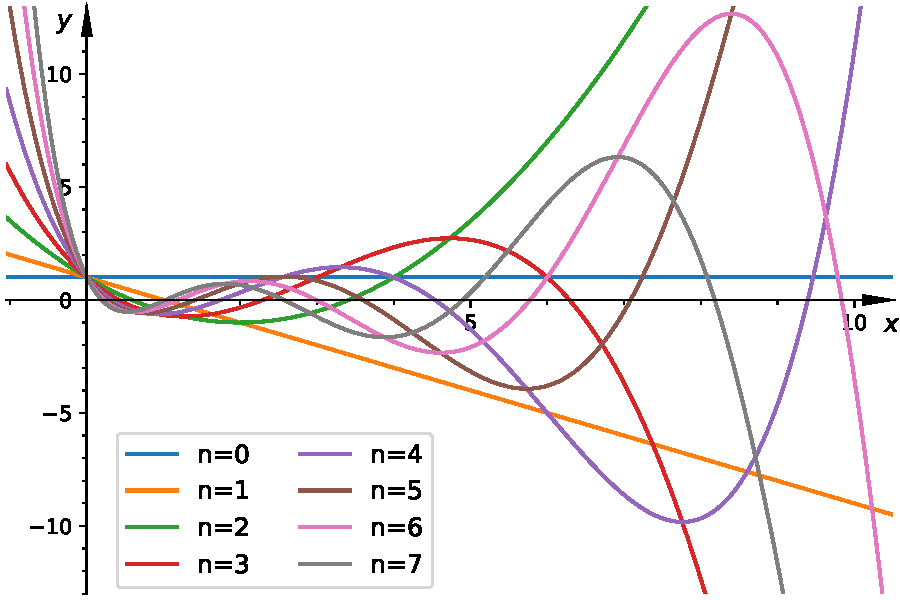
\includegraphics[width=0.7\textwidth]{%
%     papers/laguerre/images/laguerre_polynomes.eps%
% }
\caption{Laguerre-Polynome vom Grad $0$ bis $7$}
\label{laguerre:fig:polyeval}
\end{figure}

\subsection{Analytische Fortsetzung}
Durch die analytische Fortsetzung erhalten wir zudem noch die zweite Lösung der
Differentialgleichung mit der Form
\begin{align*}
\Xi_n(x)
=
L_n(x) \ln(x) + \sum_{k=1}^\infty d_k x^k
\end{align*}
Nach einigen mühsamen Rechnungen,
die den Rahmen dieses Kapitel sprengen würden,
erhalten wir
\begin{align*}
\Xi_n
=
L_n(x) \ln(x)
+
\sum_{k=1}^n \frac{(-1)^k}{k!} \binom{n}{k}
(\alpha_{n-k} - \alpha_n - 2 \alpha_k)x^k
+
(-1)^n \sum_{k=1}^\infty \frac{(k-1)!n!}{((n+k)!)^2} x^{n+k},
\end{align*}
wobei $\alpha_0 = 0$ und $\alpha_k =\sum_{i=1}^k i^{-1}$,
$\forall k \in \mathbb{N}$.
% https://www.math.kit.edu/iana1/lehre/hm3phys2012w/media/laguerre.pdf
% http://www.physics.okayama-u.ac.jp/jeschke_homepage/E4/kapitel4.pdf

%
% eigenschaften.tex -- Eigenschaften der Lösungen
% Author: Erik Löffler
%
% (c) 2020 Prof Dr Andreas Müller, Hochschule Rapperswil
%

% TODO:
%  state goal
%  use only what is necessary
%  make sure it is easy enough to understand (sentences as shot as possible)
%    -> Eigenvalue problem with matrices only
%    -> prepare reader for following examples
%
% order:
%  1. Eigenvalue problems with matrices
%  2. Sturm-Liouville is an Eigenvalue problem
%  3. Sturm-Liouville operator (self-adjacent)
%  4. Spectral theorem (brief)
%  5. Base of orthonormal functions

\section{Eigenschaften von Lösungen
\label{sturmliouville:sec:solution-properties}}
\rhead{Eigenschaften von Lösungen}

Im weiteren werden nun die Eigenschaften der Lösung eines
Sturm-Liouville-Problems diskutiert.
Im wesentlichen wird darauf eingegangen, wie die Orthogonalität der Lösungen
zustande kommt, damit diese später in den Beispielen verwendet werden kann.
Dazu wird zunächst das Eigenwertproblem für Matrizen wiederholt und angeschaut
unter welchen Voraussetzungen die Lösungen dieses Problems orthogonal sind.
Dann wird gezeigt, dass das Sturm-Liouville-Problem auch ein Eigenwertproblem
dieser Art ist und es wird auf au die Orthogonalität der Lösungsfunktionen
geschlossen.

\subsection{Eigenwertprobleme mit symmetrischen Matrizen
\label{sturmliouville:sec:eigenvalue-problem-matrix}}

% TODO: intro

Angenomen es sei eine reelle, symmetrische $n \times n$-Matrix $A$ gegeben.
Dass $A$ symmetrisch ist, bedeutet, dass
\[
    \langle Av, w \rangle
    =
    \langle v, Aw \rangle
    \qquad
    v, w \in \mathbb{R}^n
\]
erfüllt ist.

Für reelle, symmetrische Matrizen zeigt dies auch direkt, dass die Matrix
selbstadjungiert ist.
Das ist wichtig, da der Spektralsatz~\cite{sturmliouville:spektralsatz-wiki}
für selbstadjungierte Matrizen formuliert ist. Dieser sagt nun aus, dass die
Matrix $A$ diagonalisierbar ist.
In anderen Worten bilden die Eigenvektoren $v_i \in \mathbb{R}^n$ des 
Eigenwertproblems
\[
    A v_i
    =
    \lambda_i v_i
    \qquad \lambda_i \in \mathbb{R}
\]
eine Orthogonalbasis.

\subsection{Das Sturm-Liouville-Problem als Eigenwertproblem}

In Kapitel~\ref{buch:integrale:subsection:sturm-liouville-problem} wurde bereits
der Operator
\[
    L
    =
    \frac{1}{w(x)}\left( -\frac{d}{dx}p(x) \frac{d}{dx} + q(x)\right)
\]
eingeführt.
Dieser wird nun verwendet um die Differenzialgleichung 
\[
    (p(x)y'(x))' + q(x)y(x)
    =
    \lambda w(x) y(x)
\]
in das Eigenwertproblem
\begin{equation}
    \label{sturmliouville:eq:eigenvalue-problem}
    L y
    =
    \lambda y.
\end{equation}
umzuschreiben.

\subsection{Orthogonalität der Lösungsfunktionen}

Nun wird das Eigenwertproblem~\eqref{sturmliouville:eq:eigenvalue-problem} näher
angeschaut.
Um auf die Orthogonalität der Lösungsfunktion zu schliessen, wird dafür der
Operator $L$ genauer betrachtet.
Analog zur Matrix $A$ aus 
Abschnitt~\ref{sturmliouville:sec:eigenvalue-problem-matrix} kann auch für
$L$ gezeigt werden, dass dieser Operator selbstadjungiert ist, also dass
\[
    \langle L v, w\rangle
    =
    \langle v, L w\rangle
\]
gilt.
Wie in Kapitel~\ref{buch:integrale:subsection:sturm-liouville-problem} bereits
gezeigt, ist dies durch die
Randbedingungen~\eqref{sturmliouville:eq:randbedingungen} des
Sturm-Liouville-Problems sicher gestellt.

Um nun über den Spektralsatz~\cite{sturmliouville:spektralsatz-wiki} auf die
Orthogonalität der Lösungsfunktion $y$ zu schliessen, muss der Operator $L$ ein
sogenannter ''kompakter Operator'' sein.
Bei einem regulären Sturm-Liouville-Problem ist diese Eigenschaft für $L$
gegeben und wird im Weiteren nicht näher diskutiert.

Es kann nun also dank dem Spektralsatz darauf geschlossen werden, dass die
Lösungsfunktion $y$ eises regulären Sturm-Liouville-Problems eine
Linearkombination aus orthogonalen Basisfunktionen sein muss.

%%%%%%%%%%%%%%%%%%%%%%%%%%%%%% OLD section %%%%%%%%%%%%%%%%%%%%%%%%%%%%%%%%%%%%

\iffalse

\section{OLD: Eigenschaften von Lösungen
%\label{sturmliouville:section:solution-properties}
}
\rhead{Eigenschaften von Lösungen}

Im weiteren werden nun die Eigenschaften der Lösungen eines
Sturm-Liouville-Problems diskutiert und aufgezeigt, wie diese Eigenschaften
zustande kommen.

Dazu wird der Operator $L_0$ welcher bereits in
Kapitel~\ref{buch:integrale:subsection:sturm-liouville-problem} betrachtet
wurde, noch etwas genauer angeschaut.
Es wird also im Folgenden
\[
    L_0
    =
    -\frac{d}{dx}p(x)\frac{d}{dx}
\]
zusammen mit den Randbedingungen
\[
    \begin{aligned}
        k_a y(a) + h_a p(a) y'(a) &= 0 \\
        k_b y(b) + h_b p(b) y'(b) &= 0
    \end{aligned}
\]
verwendet.
Wie im Kapitel~\ref{buch:integrale:subsection:sturm-liouville-problem} bereits 
gezeigt, resultieren die Randbedingungen aus der Anforderung den Operator $L_0$
selbsadjungiert zu machen.
Es wurde allerdings noch nicht darauf eingegangen, welche Eigenschaften dies
für die Lösungen des Sturm-Liouville-Problems zur Folge hat.

\subsubsection{Exkurs zum Spektralsatz}

Um zu verstehen welche Eigenschaften der selbstadjungierte Operator $L_0$ in 
den Lösungen hervorbringt, wird der Spektralsatz benötigt.

Dieser wird in der linearen Algebra oft verwendet um zu zeigen, dass eine Matrix
diagonalisierbar ist, beziehungsweise dass eine Orthonormalbasis existiert.

Im Fall einer gegebenen $n\times n$-Matrix $A$ mit reellen Einträgen wird dazu 
zunächst gezeigt, dass $A$ selbstadjungiert ist, also dass
\[
    \langle Av, w \rangle
    =
    \langle v, Aw \rangle
\]
für $ v, w \in \mathbb{R}^n$ gilt.
Ist dies der Fall, kann die Aussage des Spektralsatzes
\cite{sturmliouville:spektralsatz-wiki} verwended werden.
Daraus folgt dann, dass eine Orthonormalbasis aus Eigenvektoren existiert,
wenn $A$ nur Eigenwerte aus $\mathbb{R}$ besitzt.

Dies ist allerdings nicht die Einzige Version des Spektralsatzes.
Unter anderen gibt es den Spektralsatz für kompakte Operatoren
\cite{sturmliouville:spektralsatz-wiki}, welcher für das
Sturm-Liouville-Problem von Bedeutung ist.
Welche Voraussetzungen erfüllt sein müssen, um diese Version des
Satzes verwenden zu können, wird hier aber nicht diskutiert und kann bei den
Beispielen in diesem Kapitel als gegeben betrachtet werden.
Grundsätzlich ist die Aussage in dieser Version dieselbe, wie bei den Matrizen,
also dass für ein Operator eine Orthonormalbasis aus Eigenvektoren existiert,
falls er selbstadjungiert ist.

\subsubsection{Anwendung des Spektralsatzes auf $L_0$}

Der Spektralsatz besagt also, dass, weil $L_0$ selbstadjungiert ist, eine
Orthonormalbasis aus Eigenvektoren existiert.
Genauer bedeutet dies, dass alle Eigenvektoren, beziehungsweise alle Lösungen
des Sturm-Liouville-Problems orthogonal zueinander sind bezüglich des
Skalarprodukts, in dem $L_0$ selbstadjungiert ist.

Erfüllt also eine Differenzialgleichung die in
Abschnitt~\ref{sturmliouville:section:teil0} präsentierten Eigenschaften und
erfüllen die Randbedingungen der Differentialgleichung die Randbedingungen
des Sturm-Liouville-Problems, kann bereits geschlossen werden, dass die
Lösungsfunktion des Problems eine Linearkombination aus orthogonalen
Basisfunktionen ist.

\fi

%
% quadratur.tex 
%
% (c) 2022 Patrik Müller, Ostschweizer Fachhochschule
%
\section{Gauss-Quadratur
  \label{laguerre:section:quadratur}}
 {\large \color{red} TODO: Einleitung und kurze Beschreibung Gauss-Quadratur}
\begin{align}
\int_a^b f(x) w(x) \, dx
\approx
\sum_{i=1}^N f(x_i) A_i
\label{laguerre:gaussquadratur}
\end{align}

\subsection{Gauss-Laguerre-Quadratur
\label{laguerre:subsection:gausslag-quadratur}}
Die Gauss-Quadratur kann auch auf Skalarprodukte mit Gewichtsfunktionen
ausgeweitet werden.
In unserem Falle möchten wir die Gauss Quadratur auf die Laguerre-Polynome
$L_n$ ausweiten.
Diese sind orthogonal im Intervall $(0, \infty)$ bezüglich
der Gewichtsfunktion $e^{-x}$.
Gleichung~\eqref{laguerre:laguerrequadratur} lässt sich wiefolgt umformulieren:
\begin{align}
\int_{0}^{\infty} f(x) e^{-x} dx
\approx
\sum_{i=1}^{N} f(x_i) A_i
\label{laguerre:laguerrequadratur}
\end{align}

\subsubsection{Stützstellen und Gewichte}
Nach der Definition der Gauss-Quadratur müssen als Stützstellen die Nullstellen
des verwendeten Polynoms genommen werden.
Das heisst für das Laguerre-Polynom $L_n$ müssen dessen Nullstellen $x_i$ und
als Gewichte $A_i$ die Integrale $l_i(x)e^{-x}$ verwendet werden.
Dabei sind
\begin{align*}
l_i(x_j)
=
\delta_{ij}
=
\begin{cases}
1 & i=j           \\
0 & \text{sonst.}
\end{cases}
\end{align*}
Laut \cite{abramowitz+stegun} sind die Gewichte also
\begin{align}
A_i
=
\frac{x_i}{(n + 1)^2 \left[ L_{n + 1}(x_i)\right]^2}
.
\label{laguerre:quadratur_gewichte}
\end{align}

\subsubsection{Fehlerterm}
Der Fehlerterm $R_n$ folgt direkt aus der Approximation
\begin{align*}
\int_0^{\infty} f(x) e^{-x} \, dx
=
\sum_{i=1}^n f(x_i) A_i + R_n
\end{align*}
un \cite{abramowitz+stegun} gibt in als
\begin{align}
R_n
=
\frac{(n!)^2}{(2n)!} f^{(2n)}(\xi)
,\quad
0 < \xi < \infty
\label{lagurre:lag_error}
\end{align}
an.

{
\large \color{red}
TODO:
Noch mehr Text / bessere Beschreibungen in allen Abschnitten
}

%
% gamma.tex -- Abschnitt über die Gamma-funktion
%
% (c) 2021 Prof Dr Andreas Müller, OST Ostschweizer Fachhochschule
%
\section{Die Gamma-Funktion
\label{buch:rekursion:section:gamma}}
\rhead{Gamma-Funktion}
Die Fakultät $x!$ kann rekursiv durch 
\[
	x! = x\cdot (x-1)! \qquad\text{und}\qquad 0!=1
\]
für alle natürlichen Zahlen $x\in\mathbb{N}$ definiert werden.
Äquivalent damit ist eine Funktion 
\begin{equation}
\Gamma(x+1) = x\Gamma(x)
\qquad\text{und}\qquad 
\Gamma(1)=1.
\label{buch:rekursion:eqn:gammadef}
\end{equation}
Kann man eine reelle oder komplexe Funktion finden, die die
Funktionalgleichung~\eqref{buch:rekursion:eqn:gammadef}
erfüllt und damit die Fakultät auf beliebige Argumente ausdehnt?

\subsection{Produktformel}
Die Fakultät $n!$ ist ein Produkt von $n$ Faktoren, es ist daher
natürlich zu versuchen, auch $x!$ als ein Produkt zu schreiben.
Allerdings kann es nicht möglich sein, dies mit einer endlichen
Anzahl von Faktoren zu machen, denn wenn $x$ grösser wird, muss auch
die Zahl der Faktoren grösser werden.
Mit jedem zusätzlichen Faktor ist ein Sprung der Werte zu erwarten.
Wir erwarten daher entweder ein unendliches Produkt oder einen
Ausdreck, bei dem die ``Anzahl'' $x$ der Faktoren im Exponenten
steht.
In diesem Abschnitt soll zunächst eine solcher Ausdruck gefunden
werden.
Dieser ist jedoch für die numerische Berechnung absolut ungeeignet,
so dass er später in ein unendliches Produkt umgeformt werden muss.

\subsubsection{Fakultät als Bruch}
Euler hat das Problem, die Fakultät auf beliebige reelle oder komplexe
Zahlen auszudehnen, wie folgt angepackt.
Zunächst hat er bemerkt, dass für ganzzahlige $x$ und natürliche $n$
\begin{align}
x! 
&=
1\cdot 2\cdot 3\cdot\ldots\cdot x
\notag
\\
&=
\frac{
1\cdot 2\cdot 3\cdot\ldots\cdot x\cdot (x+1) (x+2)\cdots(x+n)
}{
(x+1)(x+2)\cdots(x+n)
}
\notag
\\
&=
\frac{
1\cdot 2\cdot\ldots\cdot n\cdot(n+1)\cdot(n+2)\cdots(n+x)
}{
(x+1)(x+2)\cdots(x+n)
}
\notag
\\
&=
\frac{n! \cdot (n+1)(n+1)\cdots(n+x)}{(x+1)(x+2)\cdots(x+n)}
\label{buch:rekursion:gamma:eqn:fakultaet}
\end{align}
gilt.
Der Plan ist, dies so umzuformen, dass man für $x$ eine beliebige
komplexe Zahl einsetzen kann.

\subsubsection{Pochhammer-Symbol}
Die spezielle Form des Nenners und des zweiten Faktors im Zähler
von \eqref{buch:rekursion:gamma:eqn:fakultaet}
rechtfertigt die folgende Definition.

\begin{definition}[Pochhammer]
Für $a\in\mathbb{C}$ und $n\in\mathbb{N}$ heisst das Produkt
\[
(a)_n = a\cdot(a+1)\cdot(a+2)\cdots(a+n-1)
\]
das Pochhammer-Symbol oder die verschobene Fakultät.
\index{Pochhammer-Symbol}
\end{definition}

Die verschobene Fakultät $(a)_n$ hat also genau $n$ Faktoren, deren
erster $1$ ist.
Die gewöhnliche Fakultät hat $n$ Faktoren, deren erster $1$ ist, also
ist $n! = (1)_n$.

Der Ausdruck \eqref{buch:rekursion:gamma:eqn:fakultaet}
für $x!$ wird unter Verwendung des Pochhammer-Symbols zu
\begin{equation}
x! = \frac{n! (n+1)_x}{(x+1)_n}.
\label{buch:rekursion:gamma:eqn:produkt2}
\end{equation}
Leider ist dieser Ausdruck ebenfalls nicht auf beliebige $x$
verallgemeinerungsfähig, denn $(n)_x$ ist nur natürliche $x$ definiert.
Der Faktor $(n+1)_x$ enthält $x$ Faktoren beginnend bei $n$.
Für grosses $n$ sind diese Faktoren nahe beeinander, man sollte also
$(n+1)_x$ durch $n^x$ approximieren können.
Wir erweitern daher \eqref{buch:rekursion:gamma:eqn:produkt2} mit $n^x$
und erhalten
\begin{equation}
x!
=
\frac{n!\,n^x}{(x+1)_n}\cdot
\frac{(n+1)_x}{n^x}.
\label{buch:rekursion:gamma:eqn:produkt3}
\end{equation}
Der erste Faktor in diesem Ausdruck enthält jetzt nur noch Dinge,
die für beliebige $x\in\mathbb{C}$ definiert sind.

\subsubsection{Grenzwertdefinition}
Der zweite Bruch in \eqref{buch:rekursion:gamma:eqn:produkt3}
besteht aus Termen, die zwar nur für natürliches $x$ definiert sind,
wir vermuten aber, dass er für grosses $n$ gegen $1$ konvergiert.
Tatsächlich gilt
\[
\lim_{n\to\infty}
\frac{(n+1)_x}{n^x}
=
\lim_{n\to\infty}
\underbrace{\frac{n+1}{n}}_{\displaystyle\to 1}
\cdot
\underbrace{\frac{n+2}{n}}_{\displaystyle\to 1}
\cdot\ldots\cdot
\underbrace{\frac{n+x}{n}}_{\displaystyle\to 1}
=
1,
\]
da  $(n+x)/n=1+x/n\to 1$ für grosses $n$.
Dies würde die folgende Definition rechtfertigen.

\begin{definition}
\label{buch:rekursion:gamma:def:definition}
Die Gamma-Funktion $\Gamma(x)$ einer Zahl
$x\in\mathbb{C}\setminus\{0,-1,-2,-3,\dots\}$ ist der Grenzwert
\[
\Gamma(x) = \lim_{n\to\infty} \frac{n!\,n^{x-1}}{(x)_n}.
\] 
\end{definition}

\subsubsection{Rekursionsgleichung für $\Gamma(x)$}
Es ist aus der Herleitung klar, dass $\Gamma(n)=(n-1)!$ sein muss.
Wir sollten dies aber auch direkt aus der
Definition~\ref{buch:rekursion:gamma:def:definition} ableiten
können.
Dazu müssen wir nur überprüfen, ob $\Gamma(1)=0!=1$ ist und ob
die Rekursionsformel $\Gamma(n)=n\Gamma(n-1)$ gilt.

Den Wert $\Gamma(1)$ kann man direkt berechnen:
\[
\Gamma(1)
=
\lim_{n\to\infty} \frac{n!}{(1)_n}
=
\lim_{n\to\infty} \frac{n!}{n!}
=
1
\]
wegen $(1)_n=n!$.

Für die Rekursionsformel muss man den Grenzwert für $x$ und $x+1$
miteinander vergleichen.
Aus dem Term $(x+1)_n$ im Nenner muss man einen Term $(x)_n$ machen,
dies ist möglich, indem man mit $x$ erweitert:
\begin{align*}
\Gamma(x+1)
&=
\lim_{n\to\infty}\frac{n!\,n^x}{(x+1)_n}
=
x\lim_{n\to\infty}\frac{n!\,n^x}{x(x+1)_n}
=
x\lim_{n\to\infty}\frac{n!\,n^x}{(x)_{n+1}}.
\intertext{Wir müssen jetzt nur noch zeigen, dass der Grenzwert
auf der rechten Seite gegen $\Gamma(x)$ konvergiert,
in dessen Definition aber die Potenz $n^{x-1}$ vorkommt.
Wir müssen also einen Faktor $n$ los werden und gleichzeitig
aus $n$ überall $n+1$ machen, damit der Nenner wieder passt.
Dabei wird}
\Gamma(x+1)
&=
x\lim_{n\to\infty}
\frac{(n+1)!n^{x-1}}{(x)_{n+1}}
\cdot
\underbrace{\frac{n}{n+1}}_{\displaystyle\to 1}
\\
&=
x\lim_{n\to\infty}
\underbrace{\frac{(n+1)!(n+1)^{x-1}}{(x)_{n+1}}}_{\displaystyle\to\Gamma(x)}
\cdot
\frac{n^{x-1}}{(n+1)^{x-1}}
\\
&=
\Gamma(x)
\lim_{n\to\infty} \biggl(\frac{n}{n+1}\biggr)^{x-1}
=
\Gamma(x),
\end{align*}
Weil $n/(n+1)\to 1$ ist und die Funktion $z\mapsto z^{x-1}$ für alle
nach der Definition zulässigen Werte von $x$ eine stetige Funktion ist.

\subsubsection{Numerische Unzulänglichkeiten der Grenzwertdefinition}
Die Grenzwertdefinition~\ref{buch:rekursion:gamma:def:definition}
ist zwar zweifellos richtig, kann aber nicht für die numerische 
Berechnung der Gamma-Funktion verwendet werden.
Die Existenz des Grenzwertes verwendet, dass $x\ll n$ sein muss,
damit $(n+x)/n$ gegenüber $1$ vernachlässigt werden kann.
Die Grenzwertdefinition beginnt also erst, vernünftige Approximationen
von $\Gamma(x)$ zu geben, wenn $n$ viel grösser also $x$ ist.
Andererseits wächst $n!$ sehr schnell an, schon für $n=171$ ist
das Resultat grösser als was der \texttt{double}-Datentyp fassen kann.
Dies ist aber viel zu kleine, um gute Approximationen auch für kleine
Werte von $x$ zu geben.
So findet man zum Beispiel für $x=\frac12$ und $n=170$ mit Octave
\[
\frac{n!\,n^{x-1}}{(x)_n}
=
\frac{170!}{\sqrt{170}\cdot \frac12\cdot\frac32\cdot\ldots\cdot\frac{339}{2}}
=
\frac{7.2574\cdot10^{307}}{13.308\cdot 3.1381\cdot10^{305}}
=
1.7738.
\]
Andererseits werden wir später sehen, dass 
\[
\Gamma({\textstyle\frac12})
=
\sqrt{\pi}
=
1.772453850905516
\]
ist.
Die Approximation mit Hilfe der Grenzwertdefinition kann also
grundsätzlich nicht mehr als zwei korrekte Nachkommastellen liefern.

\subsubsection{Produktformel}
Ein möglicher Ausweg aus den numerischen Schwierigkeiten mit der
Grenzwertdefinition ist, den schnell wachsenden Faktor $n!$
in den Zähler zu bringen, so dass er der Konvergenz etwas nachhilft.
Wir berechnen daher den Kehrwert $1/\Gamma(x)$.

\begin{satz}
\label{buch:rekursion:gamma:satz:produktformel}
Der Kehrwert der Gamma-Funktion kann geschrieben werden als
\begin{equation}
\frac{1}{\Gamma(x)}
=
xe^{\gamma x}
\prod_{k=1}^\infty
\biggl(1+\frac{x}k\biggr)\,e^{-\frac{x}{k}},
\label{buch:rekursion:gamma:eqn:produktformel}
\end{equation}
wobei $\gamma$ die Euler-Mascheronische Konstante
\[
\gamma
=
\lim_{n\to\infty}
\biggl(\sum_{k=1}^n\frac{1}{k}-\log n\biggr)
\]
ist.
\end{satz}

\begin{proof}[Beweis]
Es sind zwei Dinge nachzuprüfen.
Zunächst muss nachgewiesen werden, dass das unendliche Produkt 
überhaupt konvergiert.
Wenn das gesichert ist, muss noch gezeigt werden, dass der Grenzwert
tatsächlich $1/\Gamma(x)$ ist.

Für die Konvergenz beachtet man, dass die Faktoren des Produkts 
die Form
\begin{align*}
\biggl(1+\frac{x}n\biggr)e^{-\frac{x}{n}}
&=
\biggl(1+\frac{x}n\biggr)
\biggl(1-\frac{x}{n}+\frac{x^2}{2n^2}-\frac{x^3}{3!n^3}+\dots\biggr)
\\
&=
1-\frac{x^2}{n^2} + 
\biggl(1+\frac{x}n\biggr)
\biggl(\frac{x^2}{2n^2}-\dots\biggr)
\\
&=
1-\frac{x^2}{n^2} + \frac{x^2}{2n^2} + O\bigl((\textstyle\frac{x}{n})^2\bigr)
\\
&=
1-\frac{x^2}{2n^2} + O\bigl((\textstyle\frac{x}{n})^3\bigr)
\end{align*}
haben.
Da die Reihe 
\[
\sum_{n=1}^\infty \frac{x^2}{n^2}
\]
konvergent ist, konvergiert auch das Produkt.
% XXX wir brauchen irgendwo das Konvergenzkriterium für ein Produkt

Um die Übereinstimmung der Produktformel mit $1/\Gamma(x)$ zu zeigen,
berechnen wir
\begin{align*}
\frac{1}{\Gamma(x)}
&=
\lim_{n\to\infty} 
\frac{(x)_n}{n!\,n^{x-1}}
=
\lim_{n\to\infty} 
\frac{x(x+1)(x+2)\cdots(x+n-1)}{1\cdot 2\cdot3\cdots (n-1)\cdot n\cdot n^{x-1}}
\\
&=
x
\lim_{n\to\infty} 
\frac{x+1}{1}
\cdot
\frac{x+2}{2}
\cdots
\frac{x+n-1}{n-1}
\cdot
n^{-x}
\\
&=
x
\lim_{n\to\infty}
\biggl(1+\frac{x}{1}\biggr)
\cdot
\biggl(1+\frac{x}{2}\biggr)
\cdots
\biggl(1+\frac{x}{n-1}\biggr)
\cdot
e^{-x\log n}
\\
&=
x
\prod_{k=1}^{n-1}
\biggl(1+\frac{x}{k}\biggr)
e^{-\frac{x}{k}}
e^{\frac{x}{k}}
e^{-x\log n}
\\
&=
x
\biggl(
\lim_{n\to\infty}
\prod_{k=1}^{n-1}
\biggl(1+\frac{x}{k}\biggr)
e^{-\frac{x}{k}}
\biggr)
\cdot
\biggl(
\lim_{n\to\infty}
e^{x\bigl(\sum_{k=1}^{n-1}\frac{1}{k} - \log n\bigr)}
\biggr)
\end{align*}
Der Klammerausdruck im Exponent des letzten Faktors auf der rechten Seite
konvergiert nach Definition der Euler-Mascheronischen Konstanten gegen
$\gamma$, somit folgt 
\[
\frac{1}{\Gamma(x)}
=
xe^{\gamma x}\prod_{k=1}^\infty \biggl(1+\frac{x}{k}\biggr)e^{-\frac{x}{k}},
\]
wie behauptet.
Damit ist Satz~\ref{buch:rekursion:gamma:satz:produktformel}
vollständig bewiesen.
\end{proof}

\begin{table}
\centering
\begin{tabular}{|>{$}c<{$}|>{$}c<{$}|>{$}c<{$}|}
\hline
k &  \Gamma(\frac12,n) & \Gamma(\frac12) - \Gamma(\frac12,n) \\
\hline
1 & 1.\underline{7}518166478 & -0.0206372031 \\
2 & 1.\underline{77}02543372 & -0.0021995137 \\
3 & 1.\underline{772}2324556 & -0.0002213953 \\
4 & 1.\underline{7724}316968 & -0.0000221541 \\
5 & 1.\underline{77245}16354 & -0.0000022156 \\
6 & 1.\underline{772453}6293 & -0.0000002216 \\
\hline
\end{tabular}
\caption{Werte $\Gamma(\frac12,n)$ von $\Gamma(\frac12)$ berechnet mit
$n=10^k$ Faktoren der
Produktformel~\eqref{buch:rekursion:gamma:eqn:produktformel}
und der zugehörige Fehler.
Die korrekten Nachkommastellen sind unterstrichen.
\label{buch:rekursion:gamma:gammatabelle}}
\end{table}

Um zu zeigen, dass die Produktform tatsächlich besser geeignet ist,
sind in der Tabelle~\ref{buch:rekursion:gamma:gammatabelle}
die Resultate der numerischen Rechnung  bis $n=1000000$ zusammengestellt.
Die Produktformel kann gute Werte von $\Gamma(x)$ auch für derart grosse
Werte von $n$ problemlos berechnen.

Der Fehler der numersichen Approximation ist von der Grössenordnung
$O(1/n)$ wie das auf Grund des verwendeten Konvergenzkriteriums
zu erwarten war.
Die Anzahl zu berücksichtigender Terme wächst daher exponentiall
mit der Anzahl gewünschter Stellen an, was für praktische Zwecke
zu langsam ist.
Für die numersiche Berechnung der Gamma-Funktion ist die Produktformel
daher im Allgemeinen nicht geeignet.

%
% Integralformel für die Gamma-Funktion
%
\subsection{Integralformel für die Gamma-Funktion}
Euler hat die folgende Integraldefinition der Gamma-Funktion gegeben.

\begin{definition}
\label{buch:rekursion:def:gamma}
Die Gamma-Funktion ist die Funktion 
\[
\Gamma
\colon
\{z\in\mathbb{C} \mid \operatorname{Re}z>0\}
\to \mathbb{C}
:
z
\mapsto
\Gamma(z) = \int_0^\infty t^{z-1}e^{-t}\,dt
\]
\end{definition}

Man beachte, dass das Integral für $x=0$ nicht definiert ist, eine
Potenzreihenentwicklung um einen Punkt $x_0$ auf der positiven reellen
Achse kann also höchstens den Konvergenzradius $\varrho=|x_0|$ haben.

\begin{figure}
\centering
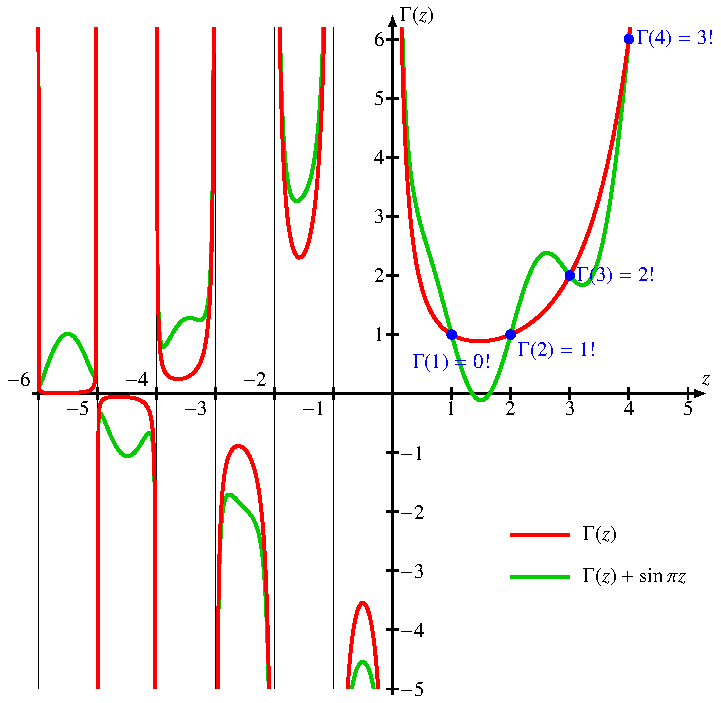
\includegraphics{chapters/040-rekursion/images/gammaplot.pdf}
\caption{Graph der Gamma-Funktion $z\mapsto\Gamma(z)$ und der alternativen
Funktion $\Gamma(z)+\sin(\pi z)$, die für ganzzahlige Argumente ebenfalls
die Werte der Fakultät annimmt.
\label{buch:rekursion:fig:gamma}}
\end{figure}

\subsubsection{Alternative Lösungen}
Die Funktion $\Gamma(z)$ ist nicht die einzige Funktion, die natürlichen
Zahlen die Werte $\Gamma(n+1) = n!$ der Fakultät annimmt.
Indem man eine beliebige Funktion $f(z)$ addiert, die auf alle
natürlichen Zahlen verschwindet, also $f(n)=0$ für $n\in\mathbb{N}$,
erhält man eine weitere Funktion, die auf natürlichen Zahlen
die Werte der Fakultät annimmt.
Ein Beispiel einer solchen Funktion ist
\begin{equation}
z\mapsto f(z)=\Gamma(z) + \sin \pi z,
\label{buch:rekursion:eqn:gammaalternative}
\end{equation}
die Funktion $f(z)=\sin\pi z$ verschwindet sogar auf allen ganzen
Zahlen.

In Abbildung~\ref{buch:rekursion:fig:gamma} ist die Gamma-Funktion
in rot geplotet, die Funktion~\eqref{buch:rekursion:eqn:gammaalternative}
in grün.
Die Punkte $(n,(n-1)!)$ sind in blau bezeichnet, sie sind beiden Graphen
gemeinsam.

\subsubsection{Pol erster Ordnung bei $z=0$}
Wir haben zu prüfen, dass sowohl der Wert $\Gamma(1)$ korrekt ist als
auch die Rekursionsformel~\eqref{buch:rekursion:eqn:gammadef} gilt.
Der Wert für $z=1$ ist
\begin{align*}
\Gamma(1)
&=
\int_0^\infty t^{1-1}e^{-t}\,dt
=
\left[ -e^{-t} \right]_0^\infty
=
1.
\end{align*}
Für die Rekursionsformel kann mit Hilfe von partieller Integration
bekommen:
\begin{align*}
\Gamma(z+1)
&=
\int_0^\infty t^{z+1-1}e^{-t}\,dt
=
\biggl[-t^{z}e^{-t}\biggr]_0^\infty
+
\int_0^\infty z t^{z-1}e^{-t}\,dt
\\
&=
z
\int_0^\infty
t^{z-1}e^{-t}\,dt
=
z \Gamma(z).
\end{align*}

Für $0<z<\varepsilon$ für eine $\varepsilon >0$ folgt aus der 
Funktionalgleichung
\[
\Gamma(z) = \frac{\Gamma(1+z)}{z}.
\]
Da $\Gamma(1)=1$ ist und $\Gamma$ eine in einer
Umgebung von $1$ stetige Funktion ist, kann sie in der Form
\(
\Gamma(1+z)=\Gamma(1) + zf(z)
\)
schreiben, wobei  $f(z)$ eine differenzierbare Funktion ist mit
$f'(1)=\Gamma'(1)$.
Daraus ergibt sich für $\Gamma(z)$ der Ausdruck
\[
\Gamma(z) = \frac{\Gamma(1)}{z} + f(z) = \frac{1}{z} + f(z).
\]
Die Gamma-Funktion hat daher and er Stelle $z=0$ einen Pol erster Ordnung.

\subsubsection{Ausdehnung auf $\operatorname{Re}z<0$}
Die Integralformel konvergiert nicht für $\operatorname{Re}z\le 0$.
Durch analytische Fortsetzung, wie sie im
Abschnitt~\ref{buch:funktionentheorie:section:fortsetzung}
beschrieben wird, kann die Funktion auf ganz $\mathbb{C}$ ausgedehnt
werden, mit Ausnahme einzelner Pole.
Die Funktionalgleichung gilt natürlich für alle $z\in\mathbb{C}$,
für die $\Gamma(z)$ definiert ist.
In einer Umgebung von $z=-n$ gilt
\[
\Gamma(z)
=
\frac{\Gamma(z+1)}{z}
=
\frac{\Gamma(z+2)}{z(z+1)}
=
\frac{\Gamma(z+3)}{z(z+1)(z+2)}
=
\dots
=
\frac{\Gamma(z+n)}{z(z+1)(z+2)\cdots(z+n-1)}
\]
Keiner der Faktoren im Nenner verschwindet in der Nähe von $z=-n$, der
Zähler hat aber einen Pol erster Ordnung an dieser Stelle.
Daher hat auch der Quotient einen Pol erster Ordnung.
Abbildung~\ref{buch:rekursion:fig:gamma} zeigt die Pole bei den
nicht negativen ganzen Zahlen.

\subsubsection{Numerische Berechnung}
\begin{table}
\centering
\begin{tabular}{|>{$}c<{$}|>{$}c<{$}>{$}c<{$}|}
\hline
k & y(10^k) & y(10^k) - \Gamma(\frac{5}{2}) \\
\hline
1 & 0.0000000000 & -0.9027452930 \\
2 & 0.3319129461 & -0.5708323468 \\
3 & 0.\underline{902}5209490 & -0.0002243440 \\
4 & 0.\underline{902745}1207 & -0.0000001723 \\
5 & 0.\underline{902745}0962 & -0.0000001968 \\
6 & 0.\underline{902745}0962 & -0.0000001968 \\
\hline
\end{tabular}
\caption{Resultate der Berechnung von $\Gamma(\frac{5}{2})$ mit Hilfe
der Differentialgleichung \eqref{buch:rekursion:gamma:eqn:gammadgl}.
Die korrekten Stellen sind unterstrichen.
Es sind immerhin sechs korrekte Stellen gefunden, wobei nur 337
Auswertungen des Integranden notwendig waren.
\label{buch:rekursion:gamma:table:gammaintegral}}
\end{table}
Im Prinzip könnte die Integraldefinition der numerischen Berechnung
entgegenkommen.
Um diese Hypothese zu prüfen, berechnen wir das Integral für
$z=\frac52$ mit Hilfe der äquivalenten Differentialgleichungen
\begin{equation}
\dot{y}(t) = t^{z-1}e^{-t}
\qquad\text{mit Anfangsbedingung $y(0)=0$}.
\label{buch:rekursion:gamma:eqn:gammadgl}
\end{equation}
Der gesuchte Wert ist der Grenzwert $\lim_{t\to\infty} y(t)$.
In der Tabelle~\ref{buch:rekursion:gamma:table:gammaintegral}
sind die Werte von $y(10^k)$ sowie die Differenzen 
$y(10^k) - \Gamma(\frac{5}{2})$ zusammengefasst.
Die Genauigkeit erreicht sechs korrekte Nachkommastellen mit nur
337 Auswertungen des Integranden.

%
% Spiegelformel
%
\subsection{Die Spiegelungsformel}

%
% Beta-Integrale
%
\subsection{Die Beta-Funktion}

\begin{definition}
Das Beta-Integral ist das Integral
\[
B(x,y)
=
\int_0^1 t^{x-1} (1-t)^{y-1}\,dt
\]
für $\operatorname{Re}x>0$, $\operatorname{Re}y>0$.
\end{definition}

Aus der Definition kann man sofort ablesen, dass $B(x,y)=B(y,x)$.
Für $y=1$ folgt ausserdem
\[
B(x,1) = \int_0^1 t^{x-1}\,dt = \biggl[ \frac{t^x}{x}\biggr]_0^1 = \frac{1}{x}.
\]
Speziell gilt $B(1,1)=1$.

\subsubsection{Rekursionsformeln für das Beta-Integral}
Aus der Definition folgt direkt
\begin{align*}
B(x,y+1)
&=
\int_0^1 t^{x-1} (1-t)^{y+1-1}\,dt
=
\int_0^1 (1-t) t^{x-1} (1-t)^{y-1}\,dt
\\
&=
\int_0^1 t^{x-1} (1-t)^{y-1}\,dt
-
\int_0^1 t^{x} (1-t)^{y-1}\,dt
\\
&=
B(x,y) - B(x+1,y)
\end{align*}
oder
\begin{equation}
B(x+1,y) = B(x,y) - B(x,y+1).
\label{buch:rekursion:gamma:betarek1}
\end{equation}
%
%XXX Vergleich mit der Rekursionsformel für Binomialkoeffizienten
%
Durch partielle Integration kann man eine weitere Rekursionsformel finden.
Dazu berechnet man
\begin{align}
B(x,y+1)
&=
\int_0^1 t^{x-1}(1-t)^{y}\,dt
\notag
\\
&=
\biggl[\frac{t^x}x(1-t)^y\biggr]_0^1
+
\frac{y}x \int_0^1 t^x(1-t)^{y-1}\,dt
\notag
\\
&=
 \frac{y}x B(x+1,y).
\label{buch:rekursion:gamma:betarek2}
\end{align}
Durch Gleichsetzen
\eqref{buch:rekursion:gamma:betarek1}
und
\eqref{buch:rekursion:gamma:betarek2}
entsteht die Rekursionsformel
\[
B(x,y)-B(x,y+1)
=
B(x+1,y)
=
\frac{x}{y}B(x,y+1)
\]
oder
\begin{equation}
B(x,y)
=
\frac{x+y}{y}B(x,y+1).
\label{buch:rekursion:gamma:betarek3}
\end{equation}

\subsubsection{Beta-Funktion und Gamma-Funktion}
Die Rekursionsbeziehung~\eqref{buch:rekursion:gamma:betarek3}
kann jetzt dazu verwendet werden, eine Darstellung der Beta-Funktion
durch die Gamma-Funktion zu finden.
Durch $n$-fache Anwendung von \eqref{buch:rekursion:gamma:betarek3}
ergibt sich zunächst
\begin{align*}
B(x,y)
&=
\frac{x+y}{y}
B(x,y+1)
=
\frac{x+y}{y}
\frac{x+y+1}{y+1}
B(x,y+2)
\\
&=
\frac{x+y}{y}
\frac{x+y+1}{y+1}
\cdot
\ldots
\cdot
\frac{x+y+n-1}{y+n-1}
B(x,y+n)
=
\frac{(x+y)_n}{(y)_n}
B(x,y+n)
\intertext{Die Beta-Funktion auf der rechten Seite kann als Integral
geschrieben werden:}
&=
\frac{(x+y)_n}{(y)_n}
\int_0^1 t^{x-1}(1-t)^{y+n-1}\,dt.
\intertext{Wir streben an, mit dem Grenzübergang $n\to\infty$ aus den
Pochhammer-Symbolen Gamma-Funktionen zu machen, dazu müssen gemäss
Definition~\ref{buch:rekursion:gamma:def:definition} weitere Faktoren
$1/(n!\,n^{x-1})$ vorhanden sein.
Wir erweitern geeignet und nehmen die übrig bleibenden Faktoren in
das Integral.
So ergibt sich}
&=
\frac{(x+y)_n}{n!\, n^{x+y-1}}
\frac{n!\,n^{y-1}}{(y)_n}
\int_0^1 n^{x} t^{x-1}(1-t)^{y+n-1}\,dt.
\intertext{Mit der Substition $s/n=t$ wird das Integral zu einem Integral
über das Interval $[0,n]$}
&=
\frac{(x+y)_n}{n!\, n^{x+y-1}}
\frac{n!\,n^{y-1}}{(y)_n}
\int_0^n
n^{x}
\biggl(\frac{s}{n}\biggr)^{x-1}
\biggl(1-\frac{s}{n}\biggr)^{y+n-1}
\,\frac{ds}{n}.
\\
&=
\frac{(x+y)_n}{n!\, n^{x+y-1}}
\frac{n!\,n^{y-1}}{(y)_n}
\int_0^n
n^{x-1}
\biggl(\frac{s}{n}\biggr)^{x-1}
\biggl(1-\frac{s}{n}\biggr)^{y+n-1}
\,ds.
\intertext{Beim Grenzübergang $n\to\infty$ wird daraus}
&=
\underbrace{\frac{(x+y)_n}{n!\, n^{x+y-1}}}_{\displaystyle \to 1/\Gamma(x+y)}
\underbrace{\frac{n!\,n^{y-1}}{(y)_n}}_{\displaystyle\to \Gamma(y)}
\int_0^n
s^{x-1}
\underbrace{\biggl(1-\frac{s}{n}\biggr)^{n}}_{\displaystyle\to e^{-s}}
\underbrace{\biggl(1-\frac{s}{n}\biggr)^{y-1}}_{\displaystyle\to 1}
\,ds.
\\
&\to \frac{\Gamma(y)}{\Gamma(x+y)} \int_0^\infty s^{x-1}e^{-s}\,ds
=
\frac{\Gamma(y)\Gamma(x)}{\Gamma(x+y)}.
\end{align*}

\begin{satz}
Die Beta-Funktion kann aus der Gamma-Funktion nach
\begin{equation}
B(x,y) = \frac{\Gamma(x)\Gamma(y)}{\Gamma(x+y)}
\end{equation}
berechnet werden.
\end{satz}

\subsubsection{Beta-Funktion und Binomialkoeffizienten}
Die Binomialkoeffizienten können mit Hilfe der Fakultät als
\begin{equation}
\binom{n}{k}
=
\frac{n!}{(n-k)!\,k!}
=
\frac{\Gamma(n-1)}{\Gamma(n-k-1)\Gamma(k-1)}
=
\frac{(n-2)\Gamma(n-2)}{\Gamma(n-k-1)\Gamma(k-1)}
=
\frac{n-2}{B(n-k-1,k-1)}
\label{buch:rekursion:gamma:binombeta}
\end{equation}
geschrieben werden.
Die Rekursionsbeziehung
\[
\binom{n+1}{k} = \binom{n}{k-1} + \binom{n}{k}
\]
der Binomialkoeffizienten erzeugt das vertraute Pascal-Dreieck,
die Formel \eqref{buch:rekursion:gamma:binombeta} für die
Binomialkoeffizienten macht daraus
\[
\frac{n-1}{B(n-k,k-1)}
=
\frac{n-2}{B(n-k,k-2)}
+
\frac{n-2}{B(n-k-1,k-1)},
\]
die für ganzzahlige Argumente gilt.
Wir wollen nachrechnen, dass dies für beliebige Argumente gilt.
\begin{align*}
\frac{(n-1)\Gamma(n-1)}{\Gamma(n-k)\Gamma(k-1)}
&=
\frac{(n-2)\Gamma(n-2)}{\Gamma(n-k)\Gamma(k-2)}
+
\frac{(n-2)\Gamma(n-2)}{\Gamma(n-k-1)\Gamma(k-1)}
\\
\frac{\Gamma(n)}{\Gamma(n-k)\Gamma(k-1)}
&=
\frac{\Gamma(n-1)}{\Gamma(n-k)\Gamma(k-2)}
+
\frac{\Gamma(n-1)}{\Gamma(n-k-1)\Gamma(k-1)}
\intertext{Durch Zusammenfassen der Faktoren im Zähler mit Hilfe
der Rekursionsformel für die Gamma-Funktion und Multiplizieren
mit dem gemeinsamen Nenner
$\Gamma(n-k)\Gamma(k-1)=(n-k-1)\Gamma(n-k-1)(k-2)\Gamma(k-2)$ wird daraus}
\Gamma(n)
&=
(k-2)
\Gamma(n-1)
+
(n-k-1)
\Gamma(n-1)
\intertext{Indem wir die Rekursionsformel für die Gamma-Funktion auf
die rechte Seite anwenden können wir erreichen, dass in allen Termen
ein Faktor
$\Gamma(n-1)$ auftritt:}
(n-1)\Gamma(n-1)
&=
(k-2)\Gamma(n-1)
+
(n+k-1)\Gamma(n-1)
\\
n-1
&=
k-2
+
n-k-1
\end{align*}


%
%
%


% %
% transformation.tex 
%
% (c) 2022 Patrik Müller, Ostschweizer Fachhochschule
%
\section{Laguerre Transformation
\label{laguerre:section:transformation}}
\begin{align}
    L \left\{ f(x) \right\}
    =
    \tilde{f}_\alpha(n)
    =
    \int_0^\infty e^{-x} x^\alpha L_n^\alpha(x) f(x) dx
    \label{laguerre:transformation}
\end{align}

\begin{align}
    L^{-1} \left\{ \tilde{f}_\alpha(n) \right\}
    =
    f(x)
    =
    \sum_{n=0}^{\infty} 
    \begin{pmatrix}
        n + \alpha \\
        n
    \end{pmatrix}^{-1}
    \frac{1}{\Gamma(\alpha + 1)}
    \tilde{f}_\alpha(n)
    L_n^\alpha(x)
    \label{laguerre:inverse_transformation}
\end{align}
% %
% wasserstoff.tex 
%
% (c) 2022 Patrik Müller, Ostschweizer Fachhochschule
%
\section{Radialer Schwingungsanteil eines Wasserstoffatoms
\label{laguerre:section:radial_h_atom}}

Das Wasserstoffatom besteht aus einem Proton im Kern 
mit Masse $M$ und Ladung $+e$.
Ein Elektron mit Masse $m$ und Ladung $-e$ umkreist das Proton
(vgl. Abbildung~\ref{laguerre:fig:wasserstoff_model}).
Für das folgende Model werden folgende Annahmen getroffen:

\begin{figure}
\centering
\includegraphics{papers/laguerre/images/wasserstoff_model.pdf}
\caption{Skizze eines Wasserstoffatoms.
Kartesische, wie auch Kugelkoordinaten sind eingezeichnet.
}
\label{laguerre:fig:wasserstoff_model}
\end{figure}

\begin{enumerate}
\item 
Das Elektron wird als nicht-relativistisches Teilchen betrachtet, 
das heisst,
relativistische Effekte sind vernachlässigbar.
\item        
Der Spin des Elektrons und des Protons
und das damit verbundene magnetische Moment
wird vernachlässigt.
\item
Fluktuationen des Vakuums werden nicht berücksichtigt.
\item
Wechselwirkung zwischen Elektron und Proton
ist durch die Coulombwechselwirkung gegeben. 
Somit entspricht die potentielle Energie der Coulombenergie $V_C(r)$
und nimmt damit die folgende Form an
\begin{align}
    V_C(r) 
    = 
    -\frac{e^2}{4 \pi \epsilon_0 r}
    \text{ mit }
    r
    =
    \lvert\vec{r}\rvert
    = 
    \sqrt{x^2 + y^2 + z^2}
    .
    \label{laguerre:coulombenergie}
\end{align}
Im Falle das der Kern einen endlichen Radius $r_0$ besitzt,
ist die $1/r$-Abhängigkeit in Gleichung \eqref{laguerre:coulombenergie}
als Näherung zu betrachten.
Diese Näherung darf nur angewendet werden, wenn die 
Aufenthaltswahrscheinlicheit des Elektrons
innerhalb $r_0$ vernachlässigbar ist.
Für das Wasserstoffatom ist diese Näherung für alle Zustände gerechtfertigt.
\item
Da $M \gg m$, kann das Proton als in Ruhe angenommen werden.
\end{enumerate}

\subsection{Herleitung zeitunabhängige Schrödinger-Gleichung}
\label{laguerre:subsection:herleitung_schroedinger}
Das Problem ist kugelsymmetrisch, 
darum transformieren wir das Problem in Kugelkoordinaten.
Somit gilt:

\begin{align*}
    r
    & =
    \sqrt{x^2 + y^2 + z^2}\\
    \vartheta
    & =
    \arccos\left(\frac{z}{r}\right)\\
    \varphi
    & =
    \arctan\left(\frac{y}{x}\right)
\end{align*}

Die potentielle Energie $V_C(r)$ hat keine direkte Zeitabhängigkeit.
Daraus folgt, dass die konstant ist Gesamtenergie $E$
und es existieren stationäre Zustände

\begin{align}
    \psi(r, \vartheta, \varphi, t)
    =
    u(r, \vartheta, \varphi) e^{-i E t / h},
\end{align}
wobei $u(r, \vartheta, \varphi)$ 
die zeitunabhängige Schrödinger-Gleichung erfüllt.

\begin{align}
    -\frac{\hbar^2}{2m} \Delta u(r, \vartheta, \varphi)
    + V_C(r) u(r, \vartheta, \varphi)
    =
    E u(r, \vartheta, \varphi)
    \label{laguerre:schroedinger}
\end{align}

Für Kugelkoordinaten hat der Laplace-Operator $\Delta$ die Form

\begin{align}
    \Delta
    =
    \frac{1}{r^2} \pdv{}{r} \left( r^2 \pdv{}{r} \right)
    + \frac{1}{r^2 \sin\vartheta} \pdv{}{\vartheta} 
    \left(\sin\vartheta \pdv{}{\vartheta}\right)
    + \frac{1}{r^2 \sin^2\vartheta} \pdv[2]{}{\varphi}
    \label{laguerre:laplace_kugel}
\end{align}

Setzt man nun 
\eqref{laguerre:coulombenergie} und \eqref{laguerre:laplace_kugel} 
in \eqref{laguerre:schroedinger} ein,
erhält man die zeitunabhängige Schrödinger-Gleichung für Kugelkoordinaten

\begin{align}
\nonumber
- \frac{\hbar^2}{2m} 
&
\left( 
\frac{1}{r^2} \pdv{}{r}
\left( r^2 \pdv{}{r} \right)
+
\frac{1}{r^2 \sin \vartheta} \pdv{}{\vartheta}
\left( \sin \vartheta \pdv{}{\vartheta} \right)
+
\frac{1}{r^2 \sin^2 \vartheta} \pdv[2]{}{\varphi}
\right)
u(r, \vartheta, \varphi)
\\
& -
\frac{e^2}{4 \pi \epsilon_0 r} u(r, \vartheta, \varphi)
=
E u(r, \vartheta, \varphi).
\label{laguerre:pdg_h_atom}
\end{align}

\subsection{Separation der Schrödinger-Gleichung}
\label{laguerre:subsection:seperation_schroedinger}


\printbibliography[heading=subbibliography]
\end{refsection}
